% Copyright (C) 2013 Columbia University in the City of New York and others.
%
% Please see the AUTHORS file in the main source directory for a full list
% of contributors.
%
% This file is part of TerraFERMA.
%
% TerraFERMA is free software: you can redistribute it and/or modify
% it under the terms of the GNU Lesser General Public License as published by
% the Free Software Foundation, either version 3 of the License, or
% (at your option) any later version.
%
% TerraFERMA is distributed in the hope that it will be useful,
% but WITHOUT ANY WARRANTY; without even the implied warranty of
% MERCHANTABILITY or FITNESS FOR A PARTICULAR PURPOSE. See the
% GNU Lesser General Public License for more details.
%
% You should have received a copy of the GNU Lesser General Public License
% along with TerraFERMA. If not, see <http://www.gnu.org/licenses/>.

\chapter{Poisson's equation on the unit square}
\label{cha:poiss-equat-unit}

\section{Problem Overview}
\label{sec:problem-formulation}

A classic problem for learning any new PDE solver package is to
consider  Poisson's equation on the unit square,  with unit
forcing and homogeneous Dirichlet boundary conditions.  The strong
form of this problem is
\begin{align}
-\nabla^2u &= f \quad\text{in } \Omega=[0,1]\times[0,1]\\
u &= 0 \quad\text{on } \partial\Omega
\end{align}
with  prescribed function, $f(x)=1$. 

To solve this problem using the Galerkin finite element method we must make a set of
additional choices. First we choose a \emph{mesh} and an \emph{element} such as
piecewise linear triangles, which together form a discrete finite
element function space $\fspace$ with suitable choice of basis
functions $\phi_{i}, i=1,\ldots n$. Any function $u\in\fspace$ is just a
linear combination of the basis functions
\begin{equation}
  \label{eq:6}
  u = \sum_{i=1}^{N} w_{i}\phi_{i}
\end{equation}
where $w_{i}$ are a set of weights that map to a discrete vector $\vec{w}$ in $\Rn$.

Next we transform the problem into its weak form by multiplying by a
test function $u_{t}$ and integrating by parts to yield the
variational problem: 
\begin{quote}
  \fbox{\parbox{.9\textwidth}{Find $u\in \fspace$ such that
  \begin{equation}
    \int_\Omega \nabla u_t\cdot \nabla u dx= \int_\Omega u_t f dx.\label{eq:weakpoisson}
  \end{equation}
  for all $u_{t} \in\fspace$.}}
\end{quote}
It is often convenient to rewrite Eq. (\ref{eq:weakpoisson}) in the
notation of linear forms as
\begin{equation}
\label{eq:linearforms}
  a(u,u_{t}) = L(u_{t})
\end{equation}
where
\begin{align}
  \label{eq:5}
  a(u,u_{t}) &= \int_\Omega \nabla u_t\cdot \nabla u dx\\
  L(u_{t})    &=  \int_\Omega u_t f dx
\end{align}
are \emph{bilinear} and \emph{linear} forms respectively.

For a linear problem, Eq. (\ref{eq:weakpoisson}) or (\ref{eq:linearforms})
assembles into the discrete linear algebra problem
\begin{equation}
  \label{eq:1}
  A\vec{w} = \vec{b}
\end{equation}
where $A$ is a matrix, $\vec{w}$ is a vector of values at the degrees
of freedom of the function space and $\vec{b}$ is a vector that is essentially the
projection of the forcing function $f$ onto $\fspace$.  We then need
to choose appropriate solvers for the linear system.

\subsection{Poisson as a non-linear problem}
\label{sec:poisson-as-non}

We could construct a model in \TF{} for this linear problem, however, as many
problems we wish to explore  quickly become non-linear, it is worth
first rephrasing this problem as a non-linear problem, and solve it
using Newton's method.  Newton can always be used for linear problems
and is guaranteed to reach a solution in exactly one iteration. % show this?

The principal idea is to rewrite our initial equation in terms of the residual
\begin{equation}
  \label{eq:2}
  r(u) = -\nabla^2 u - f
\end{equation}
which is zero, if $u$ is a solution.  The variational form of this
problem  is then:
\begin{quote}
  \fbox{\parbox{.9\textwidth}{Find $u\in\fspace$ such that
\begin{equation}
  \label{eq:3}
  F(u;u_{t}) = \int_{\Omega} u_{t}r\, dx = 0
\end{equation}
for all test functions $u_t\in\fspace$. }}
\end{quote} 
$F(u;u_{t})$ is the weak form of the (possibly non-linear) residual
and is a linear form that assembles into a vector.

For the specific case of Poisson's equation with Dirichlet boundary conditions,
the weak form of the residual can be written, after integration by
parts as
\begin{equation}
  \label{eq:4}
  F(u_{i};u_{t}) = \int_{\Omega}
  \left(
    \grad u_{t}\cdot\grad u_{i} - u_{t}f
  \right)dx
\end{equation}
where $u_{i}$ is an arbitrary function in $\fspace$.   Again, if
$u_{i}$ is a solution of the weak (or strong) form of the equations
then $F(u_{i};u_{t})=0$.  However, if  $u_{i}$ is an arbitrary
function, $F(u_{i},u_{t})$ assembles into a vector $\vec{F}$ of the
discrete residual such that $||\vec{F}||>0$.  

Our goal is to iterate on $u_{i}$\footnote{thus the subscript
$i$} until $||\vec{F}||<\mathrm{tol}$ for some norm on $||\vec{F}||$ and stopping
criterion $\mathrm{tol}$.

\subsubsection{Newton's method}
\label{sec:newtons-method}

The general idea is that given some initial guess $u_{i}$ such that
$F(u_{i}; u_{t}) \neq 0$ there is some correction $\delta u_{i}$ such
that
\begin{equation}
  \label{eq:8}
  F(u_{i} + \delta u_{i}; u_{t}) = 0
\end{equation}
Newton's method assumes we can linearize this equation such that
\begin{equation}
  \label{eq:9}
   F(u_{i} + \delta u_{i}; u_{t}) \approx F(u_{i};u_{t}) +
   J(u_{i},\delta u_{i}; u_{t})
\end{equation}
where 
\begin{equation}
  \label{eq:10}
  J(u_{i},\delta u_{i}; u_{t}) = \lim_{\epsilon\rightarrow 0}
  \frac{F(u_{i}+\epsilon\delta u_{i};u_{t}) - F(u_{i};u_{t})}{\epsilon}
\end{equation}
is the functional (Gateaux) derivative of $F$ with respect to
$u_{i}$.  After a bit of algebra, we can see that for this problem
\begin{equation}
  \label{eq:11}
  J(u_{i},\delta u_{i}; u_{t}) = \int_{\Omega} \left(
    \grad u_{t}\cdot\grad \delta u_{i} \right)dx
\end{equation}
which is a bilinear form that is equivalent to $a(\delta u_{i},u_{t})$
(Eq.\ \ref{eq:5}), which assembles into a matrix $\mat{J}$. Combining Eqs.\
(\ref{eq:8}) -- (\ref{eq:10}), Newton's method
states
\begin{quote}
  \fbox{\parbox{.9\textwidth}{while $||\vec{F}||> tol$, solve
\begin{align}
  \label{eq:12}
  J(u_{i},\delta u_{i}; u_{t}) = -F(u_{i};u_{t})
\end{align}
for $\delta u_{i}$ and update
\begin{displaymath}
u_{i+1} = u_{i} + \delta u_{i}.
\end{displaymath}}}
\end{quote}
For the purposes of the rest of this tutorial we will refer to
$F(u_{i};u_{t})$ as the ``weak form of the residual'' and
$J(u_{i},\delta u_{i};u_{t})$ as the ``weak form of the
Jacobian''.  When assembled, Eq. (\ref{eq:12}) is equivalent to the
linear algebra problem $\mat{J}\vec{\delta u} = -\vec{F}$.

\subsubsection{Writing the problem in UFL}
\label{sec:writing-problem-ufl}

The FEniCS project provides a  high level language (UFL) for describing
variational forms and finite elements that allows us to very succinctly write the
non-linear problem  as 
\begin{lstlisting}[style=UFL]
u_e = FiniteElement("Lagrange", triangle, 1)

u_i = Coefficient(u_e)
f   = Coefficient(u_e)
u_t = TestFunction(u_e)
u_a = TrialFunction(u_e)

F   = (inner(grad(u_t), grad(u_i)) - u_t*f)*dx
J   = inner(grad(u_t), grad(u_a))*dx
\end{lstlisting}
The subscripts \texttt{\_i,\_t,\_a} etc. are somewhat non-standard but
are used consistently in \TF{} to describe UFL symbols for the
\emph{iterated function}, \emph{test function}, and \emph{trial
  function}\footnote{the a is for ansatz\ldots{}} respectively.  Here we have
calculated the weak form of the Jacobian analytically. A very useful
feature of UFL, however is that it can also perform automatic
differentiation of forms and the equivalent UFL would be produced
using
\begin{lstlisting}[style=UFL]
J = derivative(F,u_i,u_a)
\end{lstlisting}
where in both descriptions, \texttt{u\_a} is the UFL symbol for the
correction $\delta u_{i}$.  

Given a description of the weak forms in UFL,  FEniCS provides the
FEniCS Form Compiler (FFC), which transforms high level UFL into
compileable C++ code using the UFC library for describing assembly of
local tensors over cells etc.  However, UFL and FFC are not sufficient
to describe the full set of choices required to construct a finite
element solution.  In FEniCS,  the \emph{DOLFIN} library (and its
python interface) provides the integration tools however, one must
construct individual applications from scratch as either python or C++
programs.  The whole purpose of \TF{} is to provide another layer of
integration that assembles the full model application from a
hierarchical options file. 

\section{Solution using \TF}
\label{sec:ch2-solution-using-tf}

To summarize,  the key choices required to fully describe and solve a
basic finite element problem using Newton's method are
\begin{enumerate}
\setlength{\itemsep}{0cm}
\item Choose a mesh
\item Choose Fields to solve $u$
\item Choose an element (Function Space)
\item Choose Initial/Boundary Conditions
\item Choose a weak form for the non-linear residual $F(u)$
\item Calculate the weak form of the Jacobian $J=F'(u)$
\item Choose a method for solving the linear problem $\mat{J}\vec{\delta u} = -\vec{F}$
\item Choose all the other adjustable parameters for controlling and
  monitoring convergence, visualization, output etc.
\end{enumerate}

The design of \TF{} is to use the SPuD library to provide a schema and interface
for managing, recording and documenting all of these choices in an
intuitive options file, from which a compiled C++ application can
be built and run.  These options files have the suffix \texttt{.tfml}
and describe the \emph{\TF{} markup language}\footnote{which is a
  flavor of  xml which should rarely  be read by humans}.  SPuD also provides the GUI
\texttt{diamond} that reads and writes \texttt{tfml} files through an
intuitive interface.  

A fully worked out description of Poisson's Equation on the unit
square with unit forcing can be found in the tutorials folder of the
installed software (by default
\texttt{\${TF\_HOME}/share/terraferma/tutorials}) in
\texttt{poisson/simple/poisson.tfml}.  To view this file, simply go to
the source folder and type
\begin{lstlisting}[style=Bash]
$ diamond poisson.tfml
\end{lstlisting}

To build and run the code:
\begin{lstlisting}[style=Bash]
$ tfbuild poisson.tfml
$ cd build
$ make run 
\end{lstlisting}
which will create a build directory \texttt{build} using
\texttt{cmake} then compile and run the code. Output from the run
includes stdout (in \texttt{terraferma.log-0)}, statistics files (see
below) and \texttt{vtk} files that can be visualized using paraview
(or any other vtk visualization system) to produce something like
\begin{figure}[h]
  \centering
  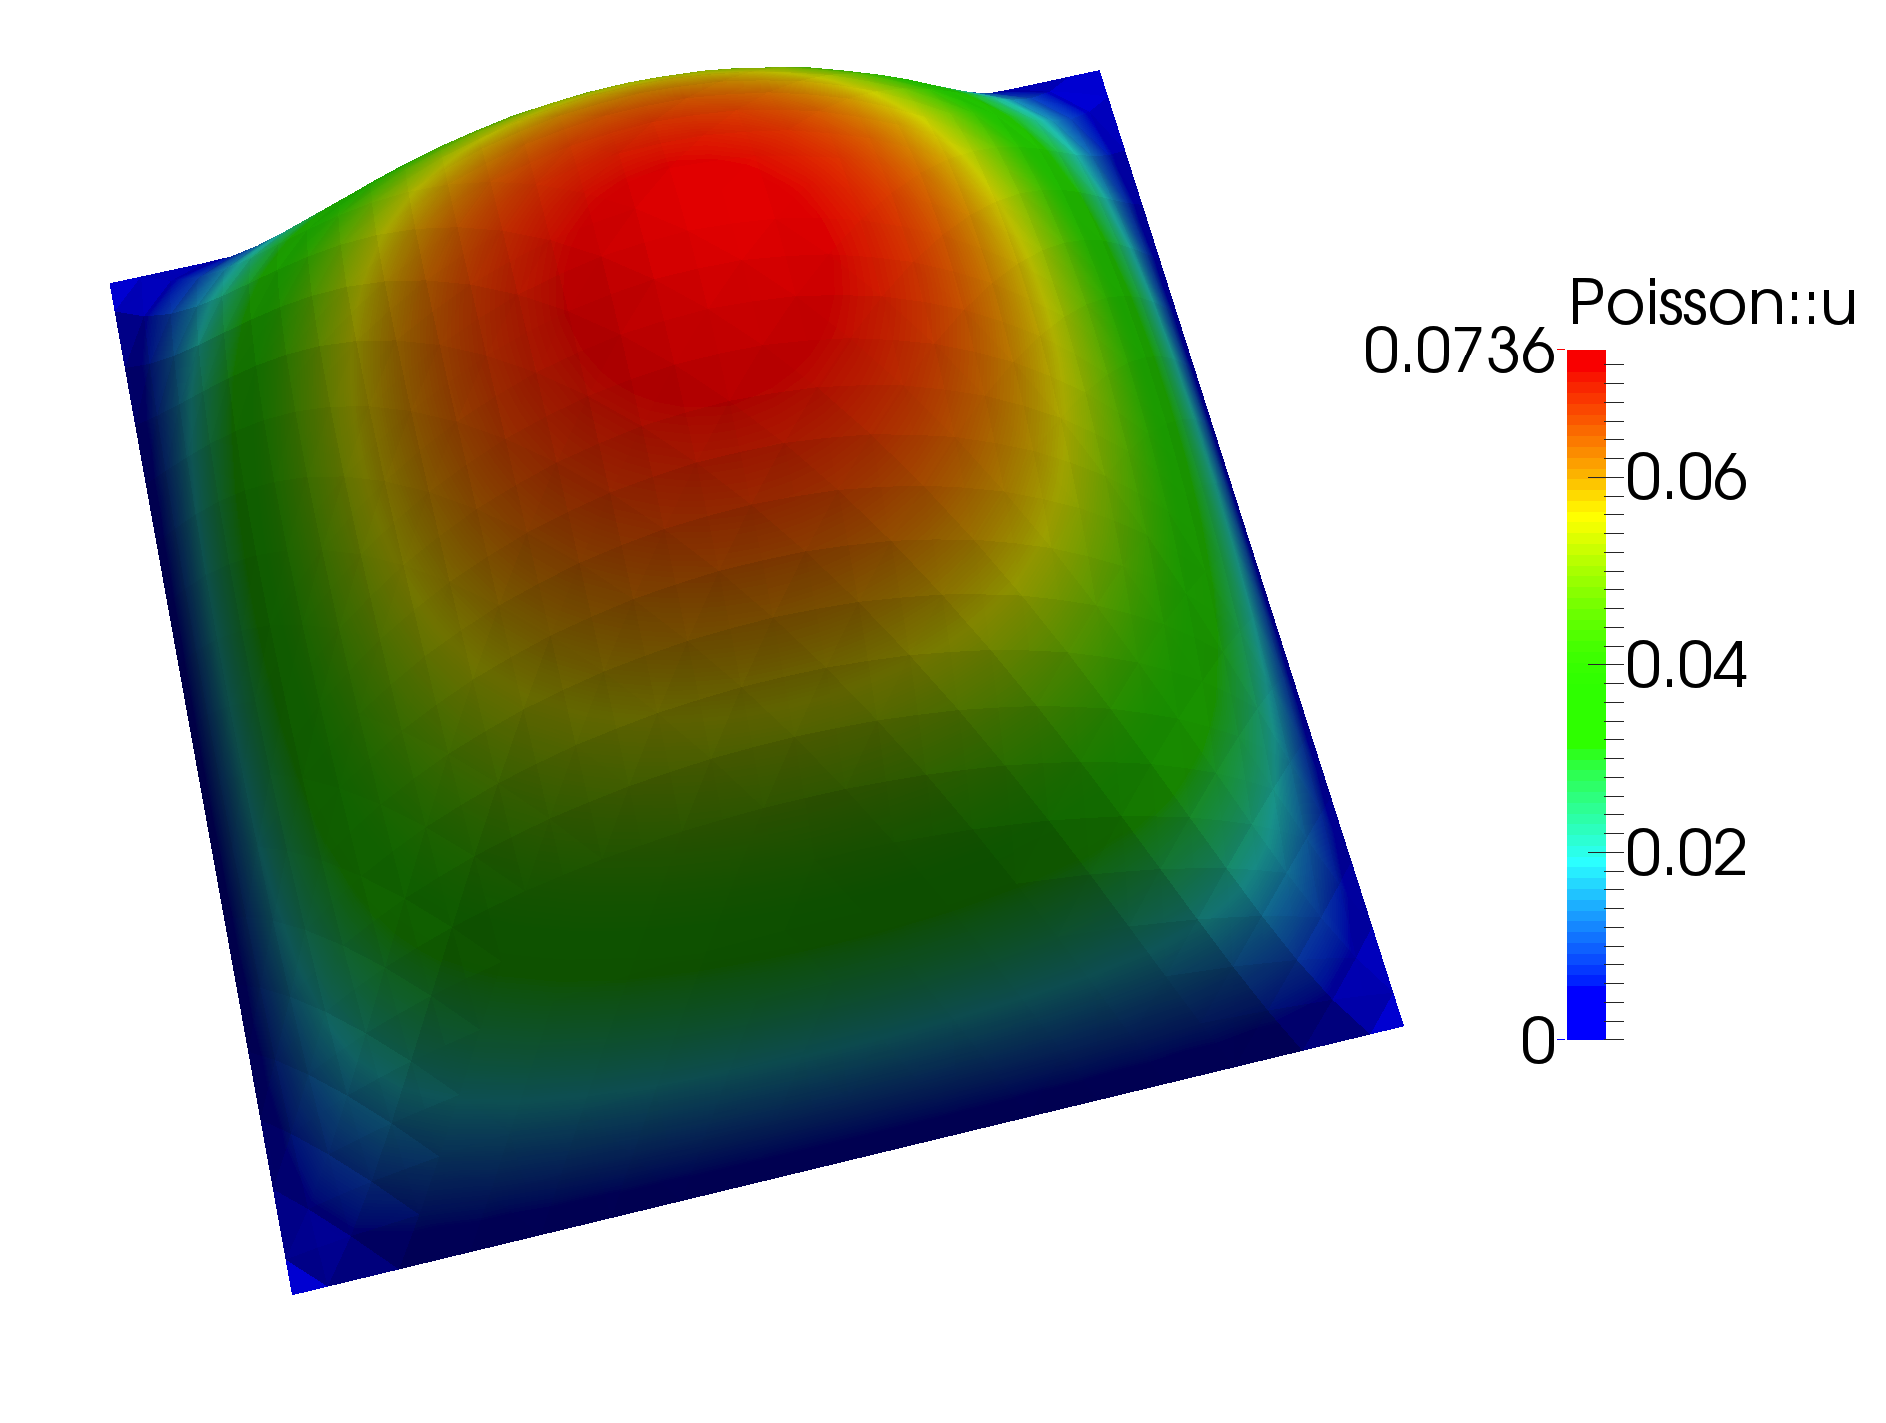
\includegraphics[width=.8\textwidth]{figures/poisson_simple.png}
  \caption{\protect\small The FEM solution of Poisson's equation on the unit square
    with unit forcing and homogeneous Dirichlet boundary conditions.
    This version solves the problem using piecewise linear elements (P1)
    on a $32\times 32$ crossed triangular mesh. The mesh can be seen
    in the facets of the solution.}
  \label{fig:simple_poisson}
\end{figure}

\subsection{Step-by-step instructions for building poisson.tfml}
\label{sec:step-step-instr}

To really begin to understand and use \TF{}, however, we need to
construct and populate our own version of \texttt{poisson.tfml} from
which we can then modify and extend later in the themes and variations
section.  Because of the graphical nature of \texttt{diamond} the
following set of steps will probably take longer to read than it
actually takes to set the problem up.  But to be completely pedantic,
here are all the steps spelled out with screen-dumps to compare.

\begin{steps}{Step}
\item  create an empty directory somewhere and start diamond
\begin{lstlisting}[style=bash]
$ mkdir mypoisson
$ cd mypoisson
$ diamond poisson.tfml & 
\end{lstlisting}%$
This will pop-up a
diamond window with an empty \texttt{tfml} file.
It should look something like
\begin{figure}[h]
  \centering
  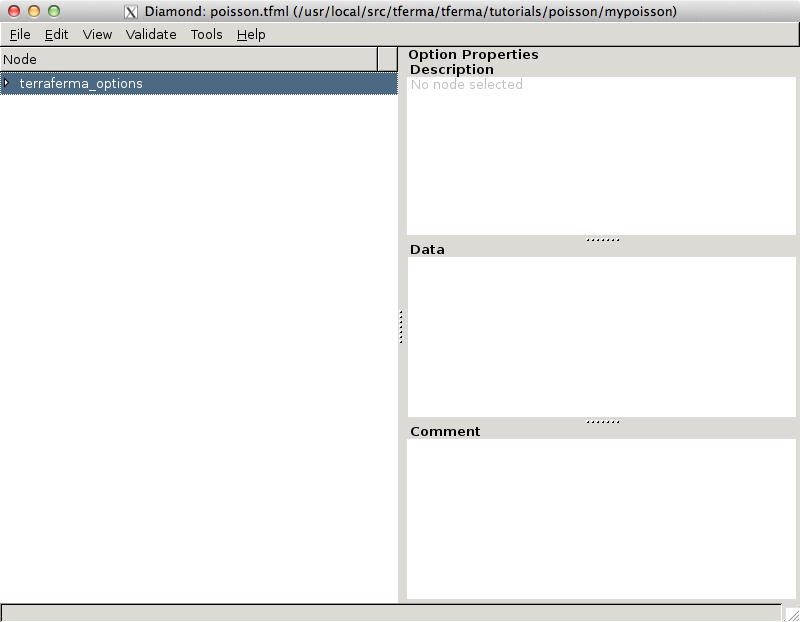
\includegraphics[width=\diamondwidth]{figures/screendumps/diamond_poisson_00.png}
  \caption{0th level diamond window}
  \label{fig:diamond-poisson-0}
\end{figure}
\pagebreak
\item Unfold the terraferma-options tab to view the top level options
  for setting \textbf{geometry}, \textbf{io}, \textbf{system}.  Required fields with
    incomplete options are highlighted in blue.
\begin{center}
  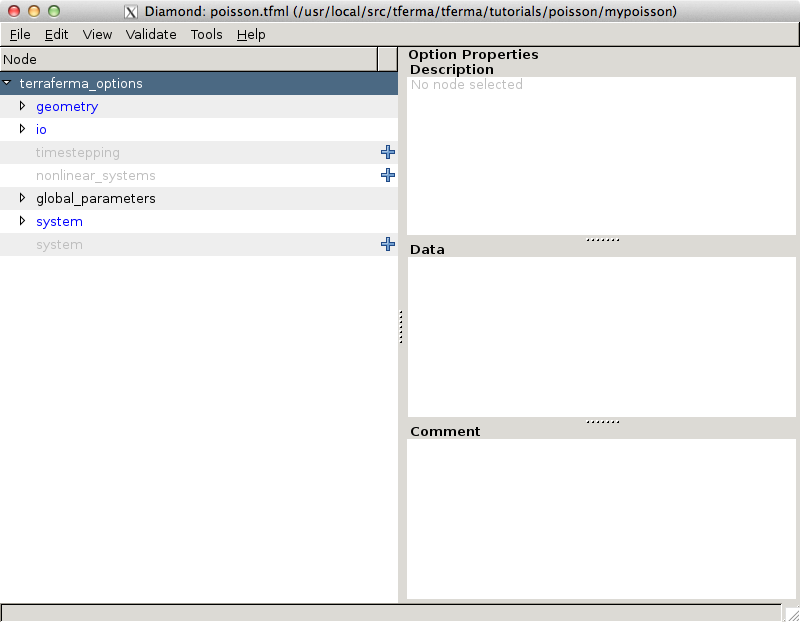
\includegraphics[width=\diamondwidth]{figures/screendumps/diamond_poisson_01.png}
\end{center}

\item\textbf{ Set Geometry option: dimension}: Unfold the
  \textbf{geometry tab} and choose \textbf{dimension}.  This is the
  physical dimension of the domain (1-D, 2-D, 3-D) and can be set only
  once (as it determines the size of other options).  In the right
  hand \textbf{data} window choose 2.
\begin{center}
  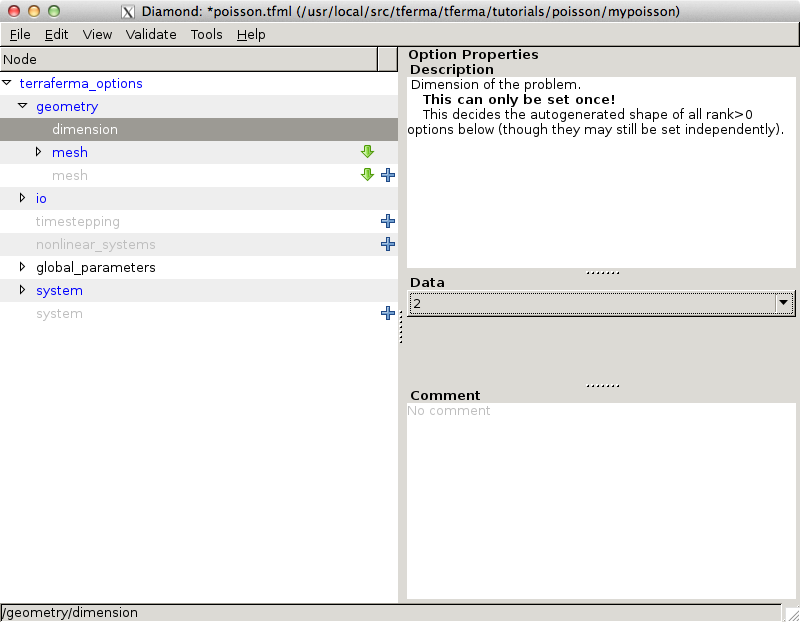
\includegraphics[width=\diamondwidth]{figures/screendumps/diamond_poisson_02a.png}    
  \end{center}

\item \textbf{Set Geometry option: Mesh} Select the Mesh tab and
  use the green arrow to choose the default name Mesh.  
  \begin{center}
    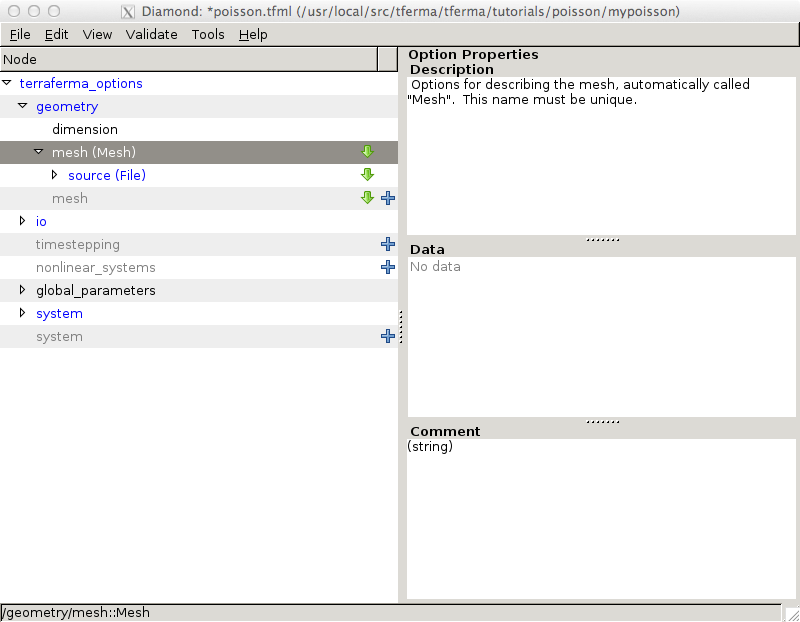
\includegraphics[width=\diamondwidth]{figures/screendumps/diamond_poisson_03a.png}
  \end{center}

Now unfold the \textbf{mesh} tab to expose the \textbf{source} tab and
using the green arrow choose \textbf{source (UnitSquare)} from the
options (default is File).
\begin{center}
  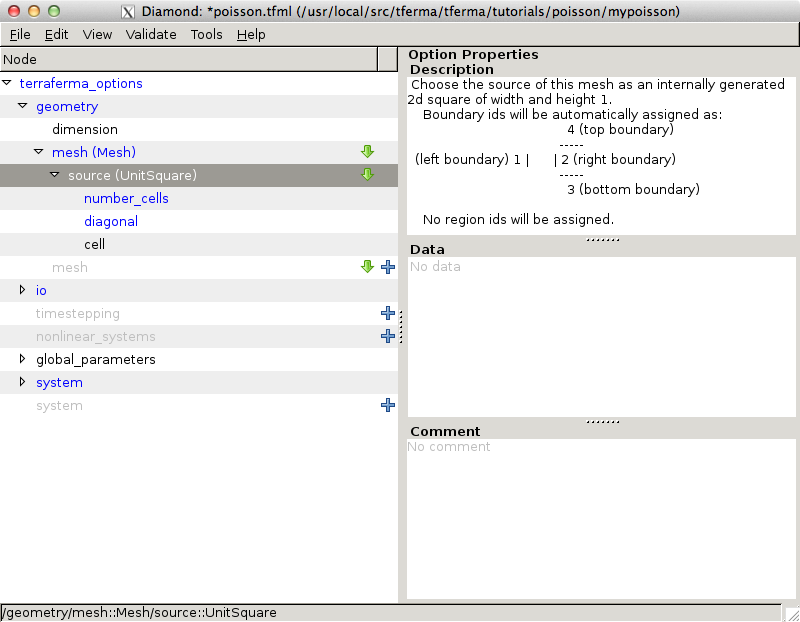
\includegraphics[width=\diamondwidth]{figures/screendumps/diamond_poisson_03b.png}
\end{center}
This will expose two more fields, \textbf{number\_cells} and
\textbf{diagonal}.

Choose \textbf{number\_cells} and set each field to 32 (for a
$32\times32$ cell mesh).
\begin{center}
    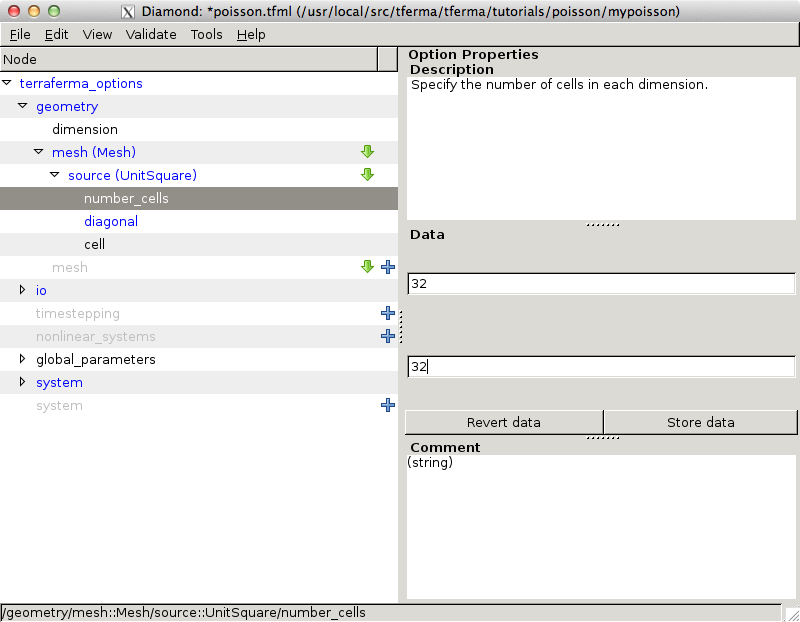
\includegraphics[width=\diamondwidth]{figures/screendumps/diamond_poisson_03c.png}
\end{center}

Then choose \textbf{diagonal} and set to \textbf{right/left}. 
\begin{center}
    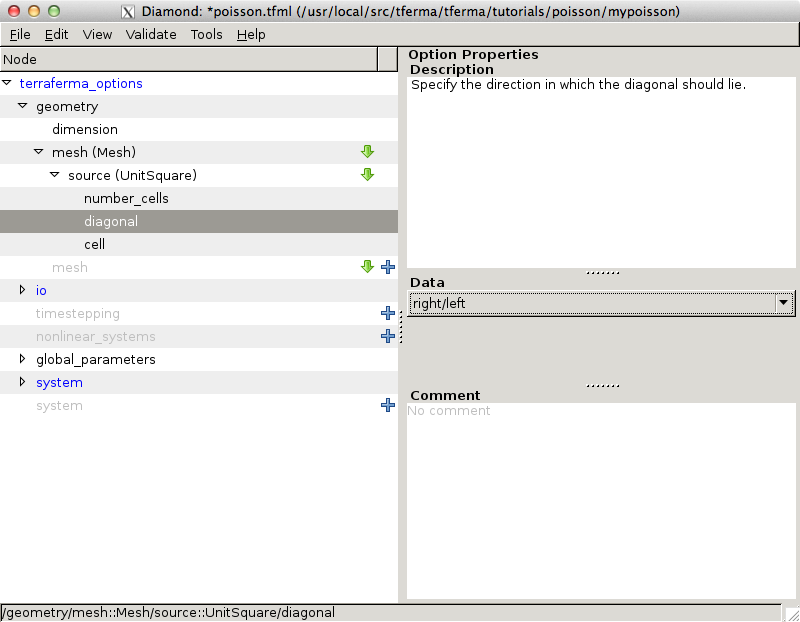
\includegraphics[width=\diamondwidth]{figures/screendumps/diamond_poisson_03d.png}
\end{center}
This completes all the required choices for setting the geometry and
the geometry tab should have changed from blue to black. At this point
(or before) you should save your file (and you can refold the geometry
tab). Also hopefully by this point it
  should be relatively clear how to maneuver around the diamond
  window.  
\item \textbf{Setting io parameters:}  The next step is to set IO
  parameters.
First unfold both the \textbf{io} then \textbf{visualization} tabs.
\textbf{output\_base\_name} is a required field and should be blue. It sets the
root-name of any output file.  Set this to \emph{poisson}.
\textbf{Caution!} do not include a line return after the string poisson. 
\begin{center}
    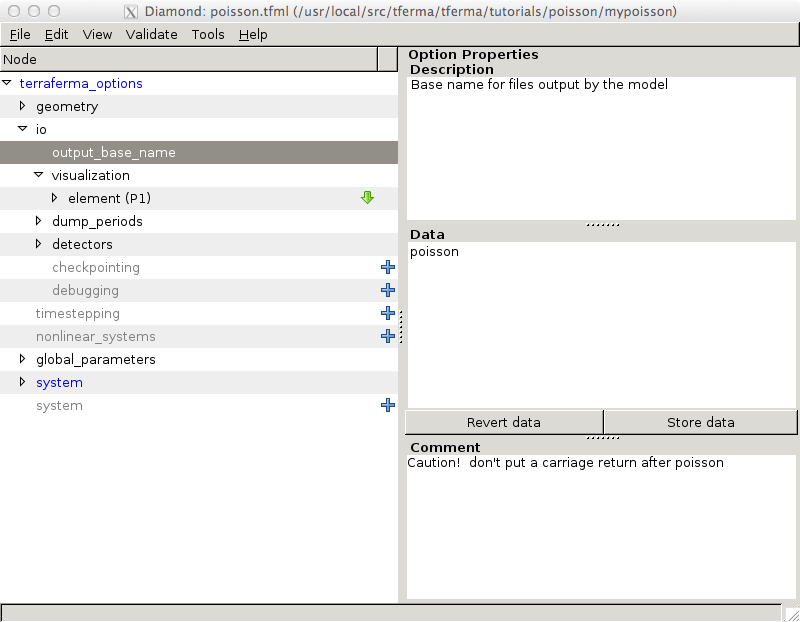
\includegraphics[width=\diamondwidth]{figures/screendumps/diamond_poisson_04.png}
\end{center}
\textbf{visualization} sets the default element used in the vtk files
for visualizing fields.  This is optional and defaults to P1 (piecewise
linear functions) which will be adequate for this problem which will
also use P1 elements.

This completes the \textbf{io} options tree.
%{\samepage
\item \textbf{Setting the System:}  The \textbf{system} is the heart of
  \TF{} and includes all the choices of fields, elements,
  coefficients, boundary
  conditions and solvers.  You can have multiple systems in any
  problem but each one needs a \textbf{name}, a \textbf{mesh} and a
  \emph{unique}, global \textbf{ufl\_symbol}.  Start by setting the system
  name to \texttt{poisson}.
\textbf{Note!}  For any name field you will need to hit return in
diamond to set it,  other fields you should not include carriage returns. 
\begin{center}
    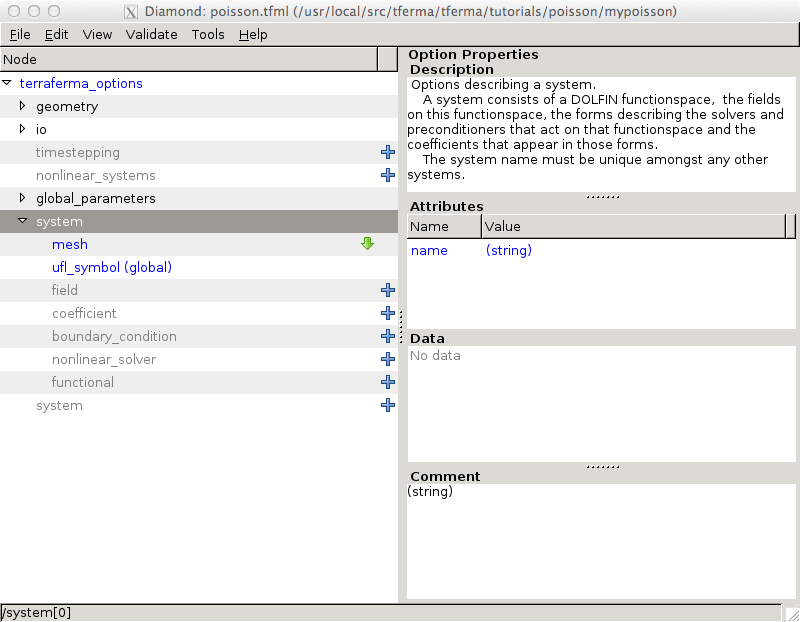
\includegraphics[width=\diamondwidth]{figures/screendumps/diamond_poisson_05a.png}
\end{center}
then choose  the \textbf{mesh} name to be consistent with what you set in
geometry (Mesh), and choose \textbf{ufl\_symbol (global)} and set it to
\texttt{us}. (Later on we will distinguish between system symbols
which include all fields in a system, and the individual field
symbols).
\begin{center}
    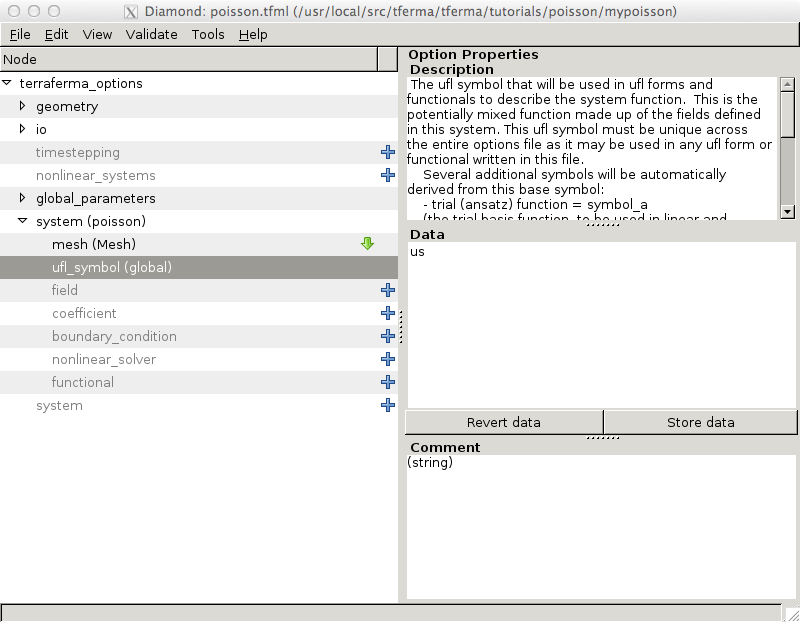
\includegraphics[width=\diamondwidth]{figures/screendumps/diamond_poisson_05c.png}
\end{center}
%}
\item \textbf{Setting the field:} Next step is to actually describe
  the field (function) or fields we are trying to solve in each
  system.  Poisson has only one field and which we will enable by
  clicking the $+$ next to the greyed out \textbf{field} tab and
  unfold the new field tab.
\begin{center}
    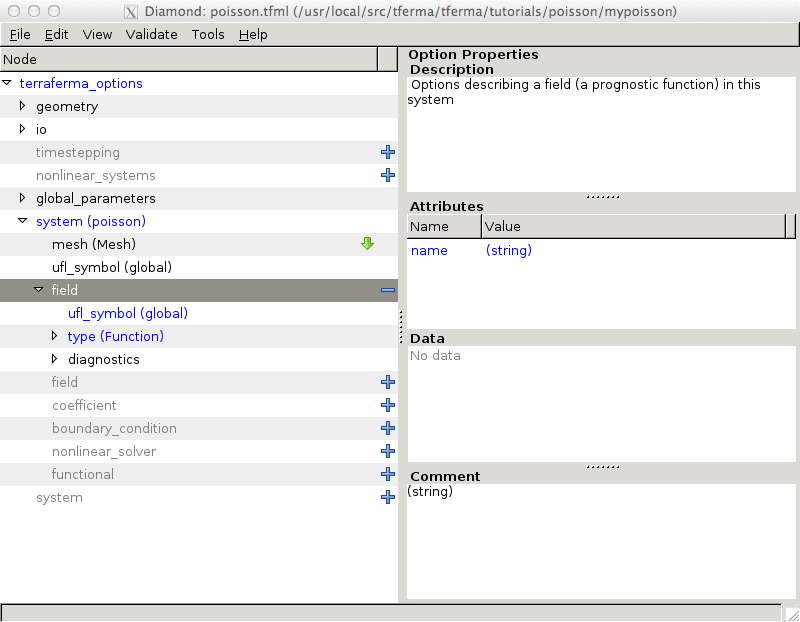
\includegraphics[width=\diamondwidth]{figures/screendumps/diamond_poisson_06a.png}
\end{center}
Each field requires both a \textbf{name} and a unique, global
\textbf{ufl\_symbol}.  Here set the field name to \texttt{ufield} and
the ufl\_symbol (global) to \texttt{u}.
\begin{center}
    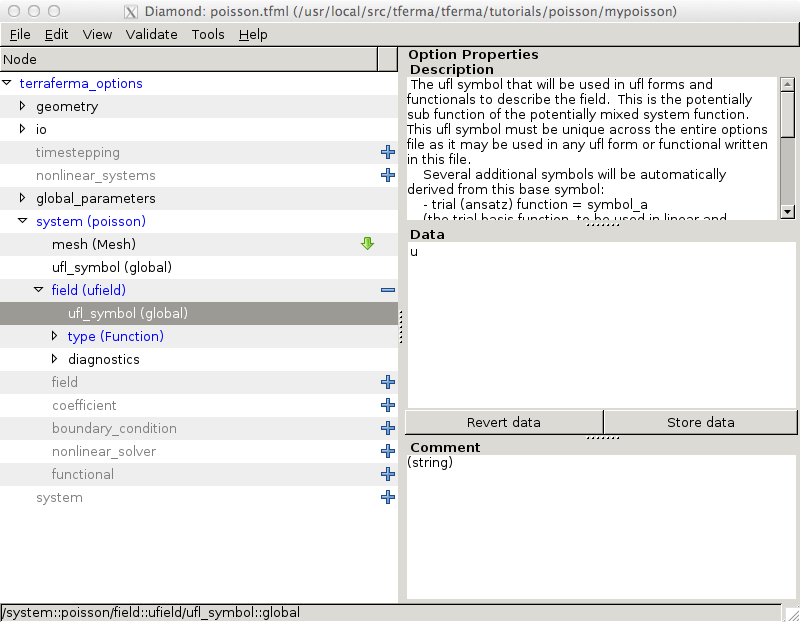
\includegraphics[width=\diamondwidth]{figures/screendumps/diamond_poisson_06c.png}
\end{center}
\item \textbf{Setting Field attributes:} Once named we next need to
  set critical attributes on the field including its \textbf{rank}
  (scalar, vector or tensor valued field), the \textbf{element},
  \textbf{initial conditions} and \textbf{boundary conditions.} Unfold
  the \textbf{Function} tab and its sub tab \textbf{rank}
\begin{center}
    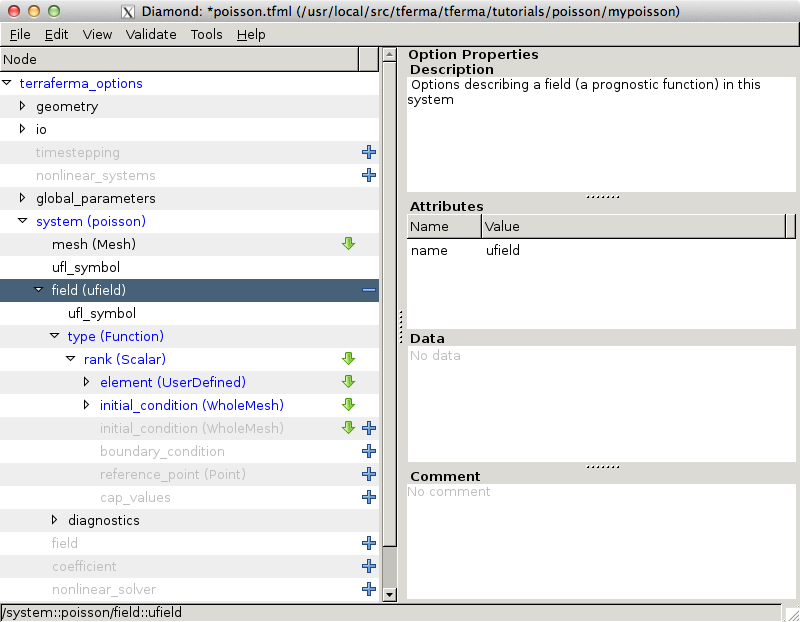
\includegraphics[width=\diamondwidth]{figures/screendumps/diamond_poisson_07a.png}
\end{center}
\textbf{rank} is already set to Scalar (green arrows could choose
vector or tensor). Use the green arrows to choose the built in
\textbf{element} P1 (which automatically chooses an element family
``CG'' (continuous Galerkin, or Lagrange element) of degree 1.
\begin{center}
    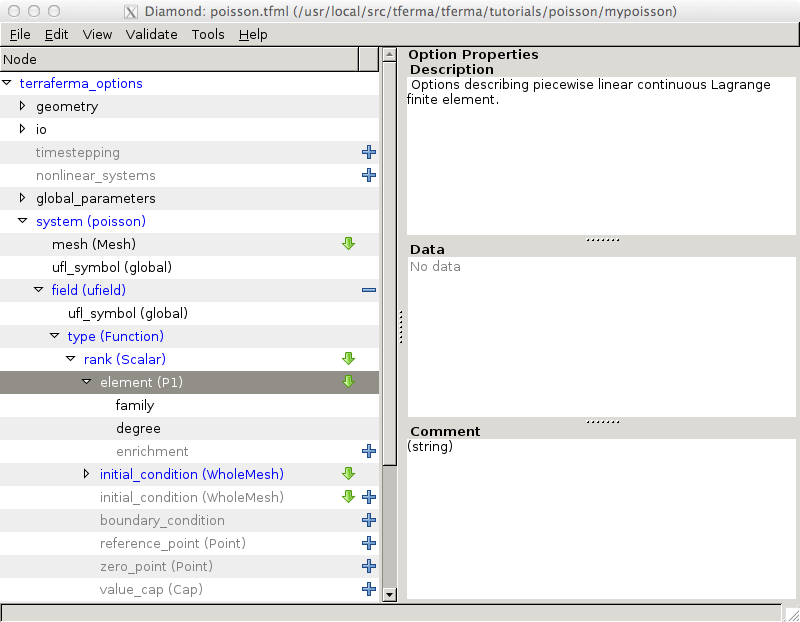
\includegraphics[width=\diamondwidth]{figures/screendumps/diamond_poisson_07b.png}
\end{center}
\item \textbf{Setting initial conditions:} Because we
  often use iterative solvers even on steady state problems, we need
  to initialize all fields with an initial condition.  Here we will
  just set it to a constant 0 over the whole mesh.  Unfold the
  \textbf{initial\_condition (WholeMesh)} tab and set the constant to
  \texttt{0.}
\begin{center}
    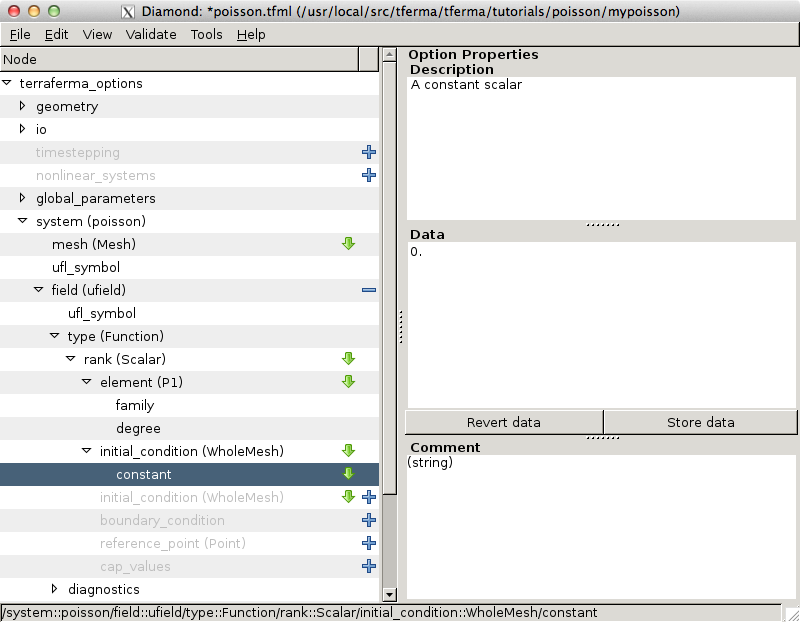
\includegraphics[width=\diamondwidth]{figures/screendumps/diamond_poisson_07c.png}
\end{center}
\item \textbf{Setting Boundary conditions:} Now we need to set
  Dirichlet conditions on the field so that it is zero on all four
  boundaries. First, activate the \textbf{boundary\_condition} tab,
  give it a name (\texttt{ZeroBCs}) and
  unfold all the sub-options. 
\begin{center}
    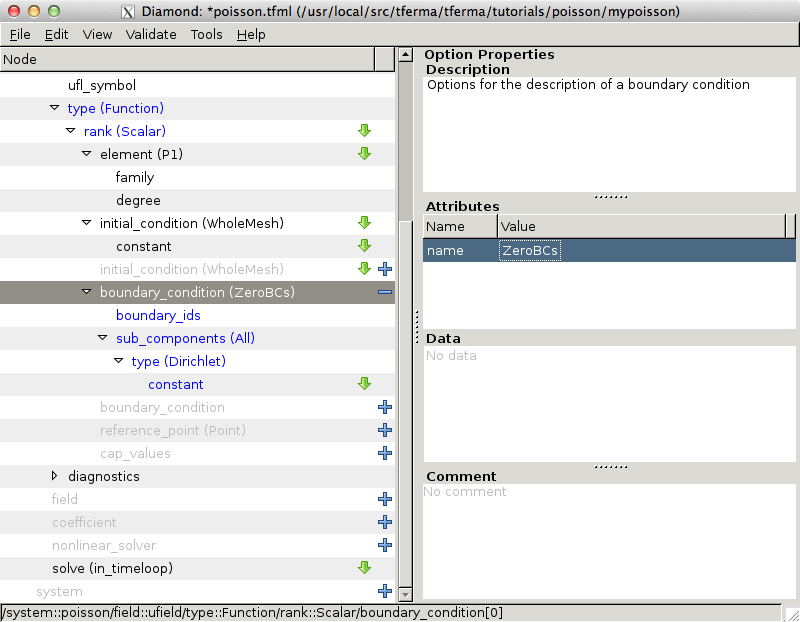
\includegraphics[width=\diamondwidth]{figures/screendumps/diamond_poisson_08b.png}
\end{center}
This will expose the options \textbf{boundary\_ids} which identify
which boundaries are affected, and \textbf{Type (Dirichlet)} which
let's you set a function that evaluates the Dirichlet BCs.  For the
unit square,  the Boundary ID's are shown with the \textbf{source
  (UnitSquare)} tab (see Step 4, second figure).  Here we'll set all
of them by putting \texttt{1 2 3 4} in \textbf{boundary\_ids}.  
\begin{center}
    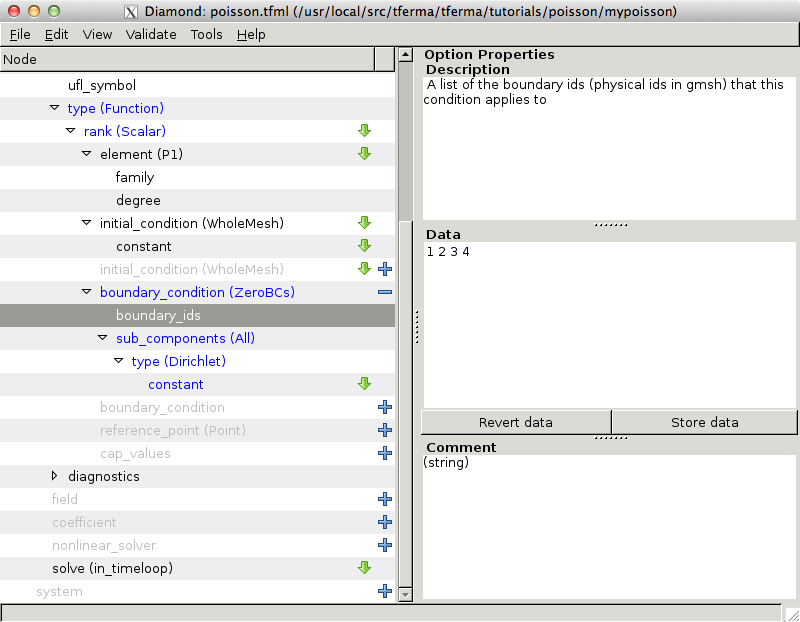
\includegraphics[width=\diamondwidth]{figures/screendumps/diamond_poisson_08c.png}
\end{center}
and we will set the \texttt{type (Dirichlet)} to a constant function
with value 0.
\begin{center}
    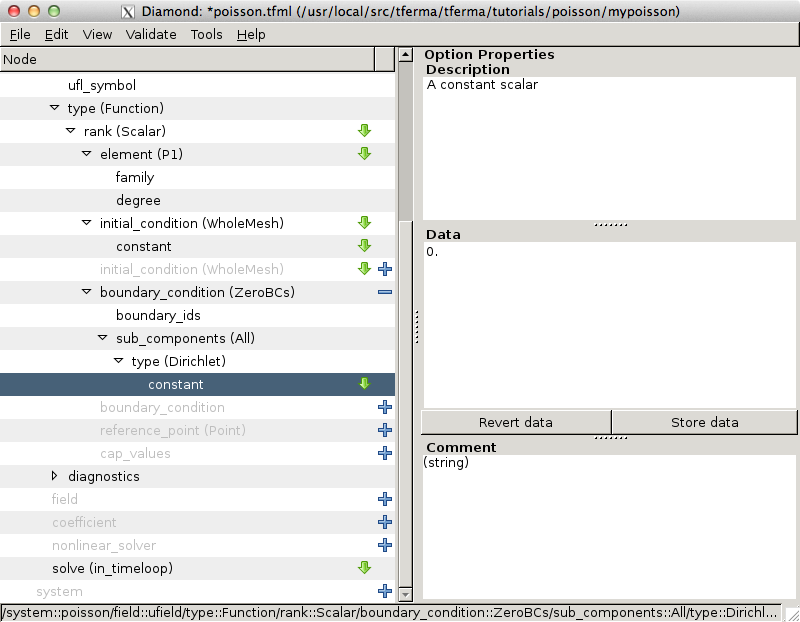
\includegraphics[width=\diamondwidth]{figures/screendumps/diamond_poisson_08d.png}
\end{center}
This completes the \textbf{Function} tab, which you can refold.
\item \textbf{Setting Diagnostics on a field:}  If you want to actually visualize
  or get output about a field, you'll need to add it to the
  diagnostics.  Unfold the \textbf{diagnostics} tab and activate
  \textbf{include\_in\_visualization} and
  \textbf{include\_in\_statistics}. Other options are available.
\begin{center}
    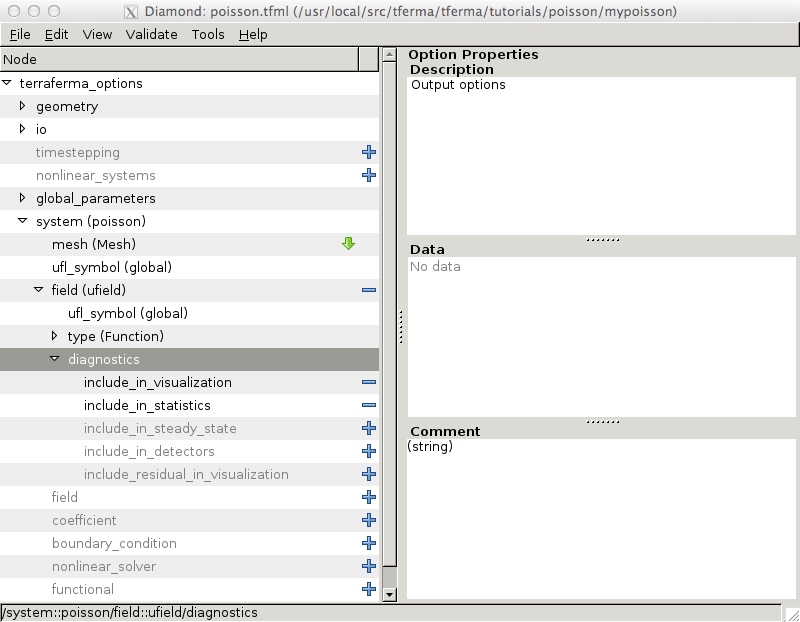
\includegraphics[width=\diamondwidth]{figures/screendumps/diamond_poisson_09.png}
\end{center}
This completes the \textbf{field} tab
\item \textbf{Setting the RHS coefficient $f$:} To solve Poisson, we
  need to give the system a RHS function $f(\vec{x})$ which in this
  case is a constant $f=1$.  In ufl notation,  $f$ is a
  \emph{coefficient} in the form that can be evaluated at any point in
  the domain.  To set $f$, activate the \textbf{coefficient} tab and
  give it a name (here \texttt{rhs}) and unfold. We will also need to
  give it a  ufl symbol (\texttt{f}). 
\begin{center}
    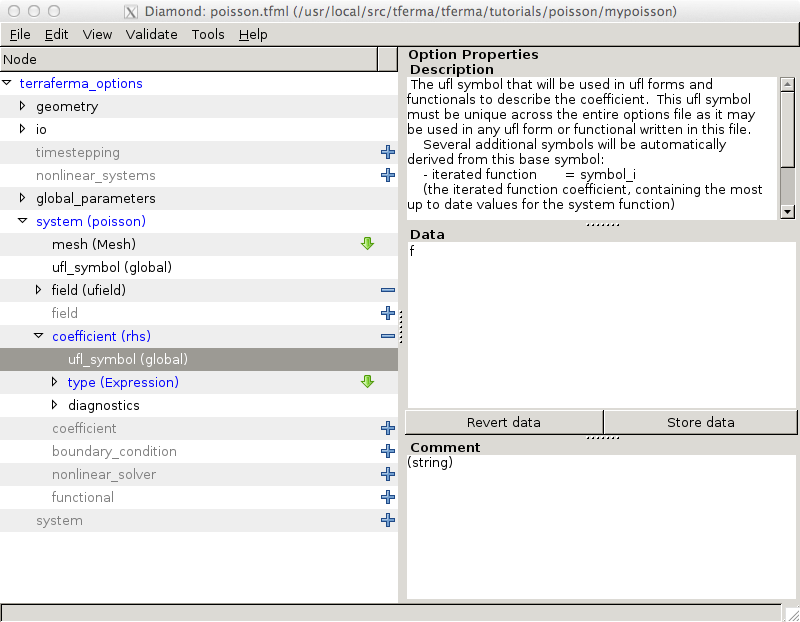
\includegraphics[width=\diamondwidth]{figures/screendumps/diamond_poisson_10b.png}
\end{center}
 To evaluate \texttt{f}, we need to set the \textbf{type} to
\textbf{Constant} using the drop down arrows, then continue to unfold
until you can set the constant value to 1.
\begin{center}
    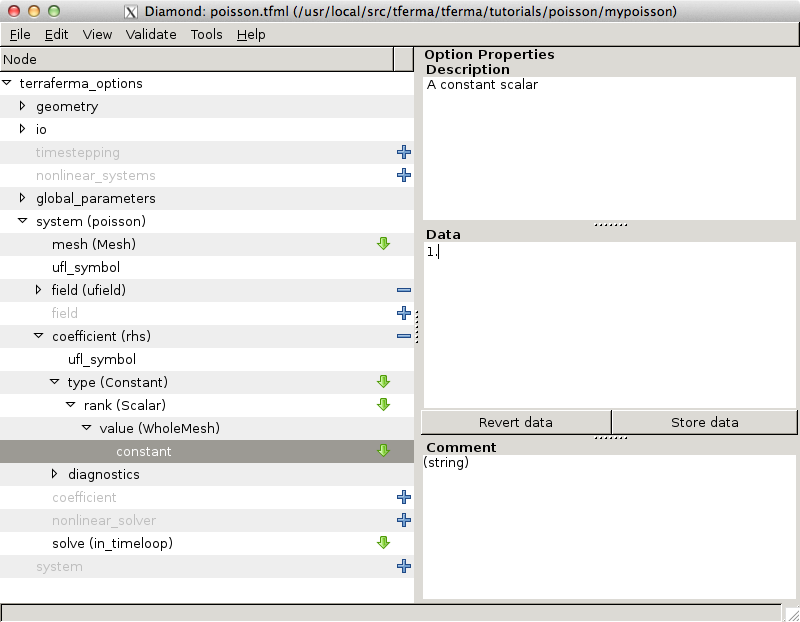
\includegraphics[width=\diamondwidth]{figures/screendumps/diamond_poisson_10c.png}
\end{center}
This completes the coefficient field.
\item \textbf{Setting the solver (and equations):}  The last set of
  choices involve setting the solvers for the system.  In \TF{}, the
  actual equations we want to solve are part of the solver as each
  solver acts as an operator over the fields (and you can have
  multiple solvers in a system).  Here we will implement Poisson using
  PETSc's Newton solver SNES.  

Start by activating the \textbf{nonlinear\_solver} tab, name the
solver (\texttt{Solver}) and unfold.
\begin{center}
    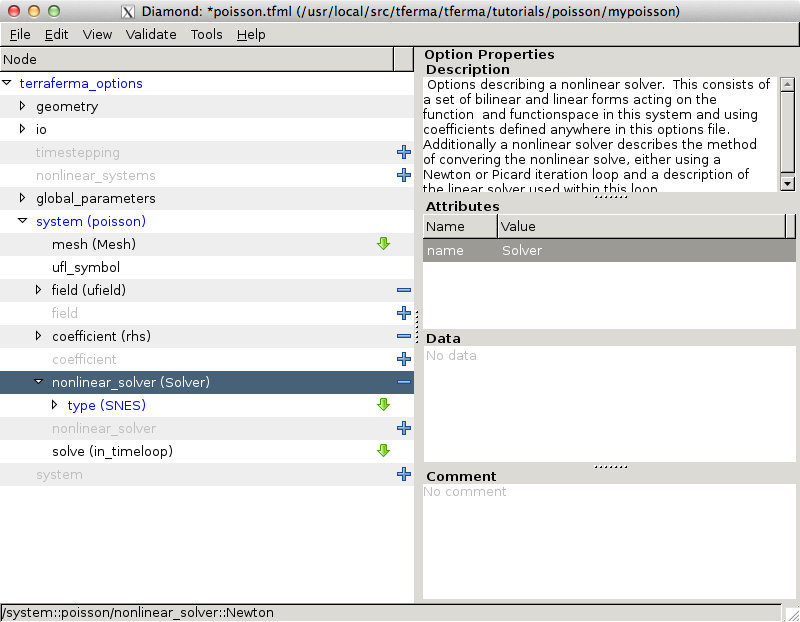
\includegraphics[width=\diamondwidth]{figures/screendumps/diamond_poisson_11a.png}
\end{center}
We will use the default type \textbf{SNES} which is PETSc's Scaleable
Non-linear Equation Solver which provides a large range of Newton and
quasi-newton schemes with control.
\item \textbf{Setting the SNES options:} Unfold the \textbf{type
    (SNES)} tab to show all the required options for a non-linear
 Newton  solver
\begin{center}
    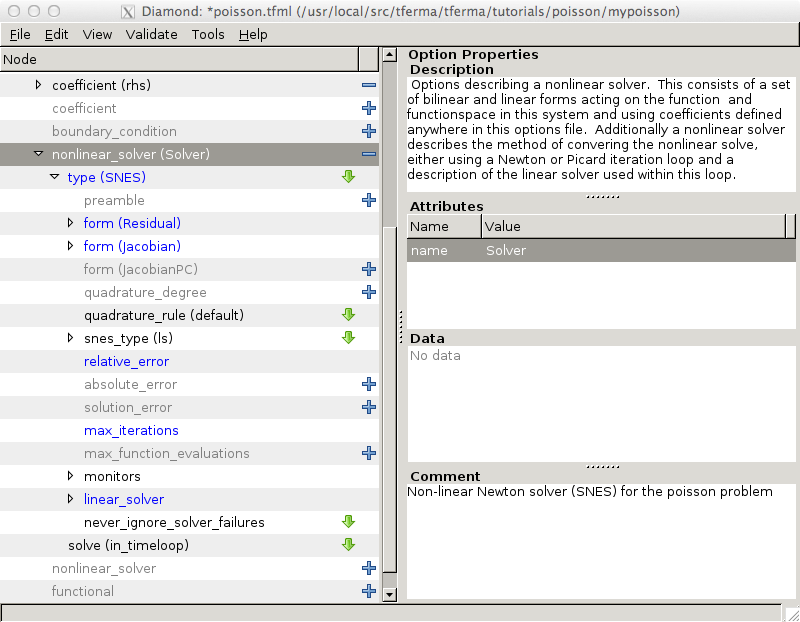
\includegraphics[width=\diamondwidth]{figures/screendumps/diamond_poisson_11b.png}
\end{center}
which include weak forms for the \textbf{Residual}, and
\textbf{Jacobian}, parameters to control convergence such as
\textbf{relative\_tolerance} and \textbf{maximum\_iterations} as well
as choice of \textbf{linear\_solvers} for the inner solver.

First we will set the weak form for the \textbf{form (Residual)}.
First highlight the  \textbf{form (Residual)} tab and in the
\textbf{Data} window add the following piece of ufl
\begin{lstlisting}[style=ufl]
F   = (inner(grad(u_t), grad(u_i)) - u_t*f)*dx
\end{lstlisting}
to define the weak form of the residual given on field \texttt{u} and
coefficient \texttt{f}.  The subscripted ufl symbols are automatically
generated by \TF{}. 
\begin{center}
    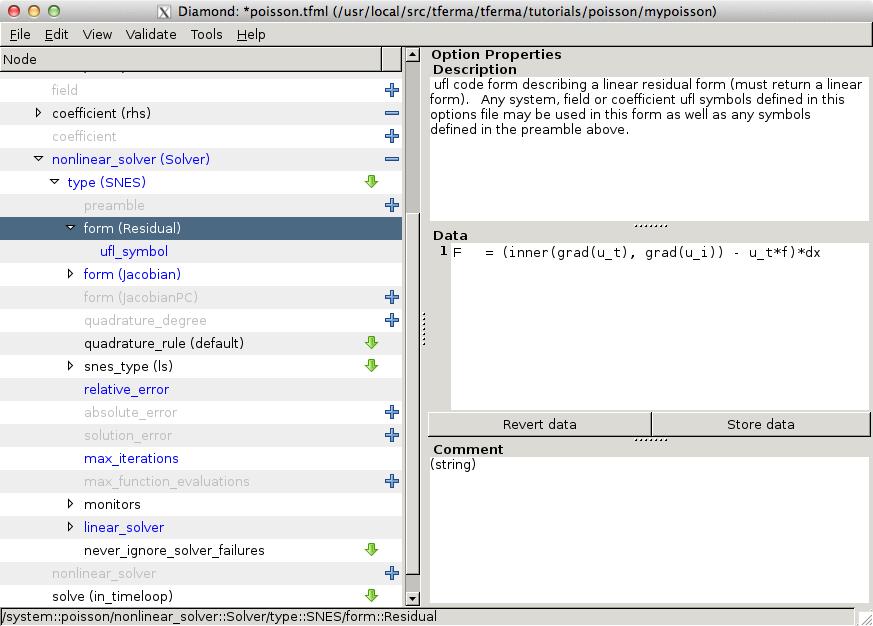
\includegraphics[width=\diamondwidth]{figures/screendumps/diamond_poisson_11c.png}
\end{center}
Also unfold the \textbf{form (Residual)} tab and set the
\textbf{ufl\_symbol (solver)} for the form to \texttt{F}.  Note
\textbf{ufl\_symbol (solver)} need only be unique within a solver,
thus you can have many solvers with different residuals all named \texttt{F}.

To set the Jacobian choose  the \textbf{form (Jacobian)} tab and add
the ufl
\begin{lstlisting}[style=ufl]
J = derivative(F,us_i,us_a)
\end{lstlisting}
and set its \textbf{ufl\_symbol (solver)} to \texttt{J}.  Note the derivative is taken
with respect to the \textbf{System} ufl symbol \texttt{us} not the
field (this will become more obvious with other problems).
\begin{center}
    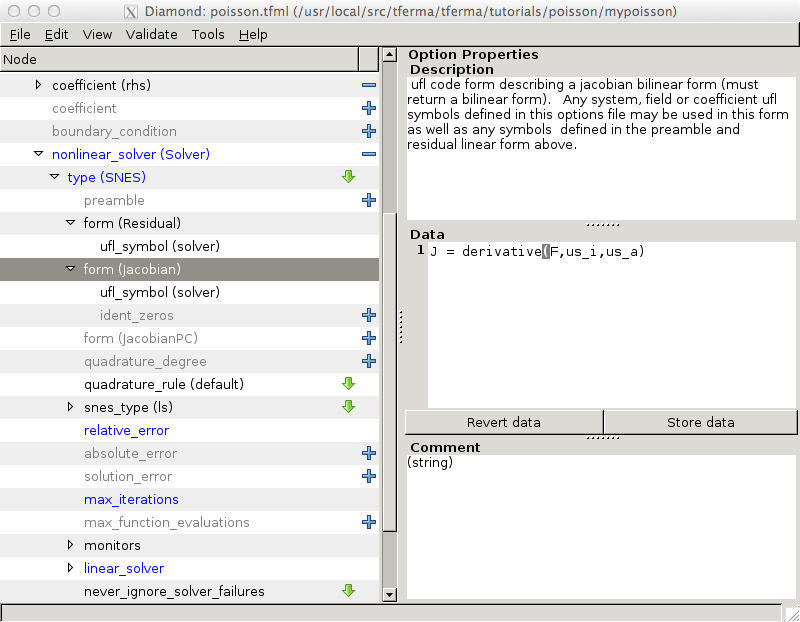
\includegraphics[width=\diamondwidth]{figures/screendumps/diamond_poisson_11d.png}
\end{center}

Now set \textbf{relative\_error} to \texttt{1.e-6} and
\textbf{max\_iterations} to \texttt{20} (and we won't need more than 1
actually for this problem) and unfold the \textbf{linear\_solver} tab
\begin{center}
    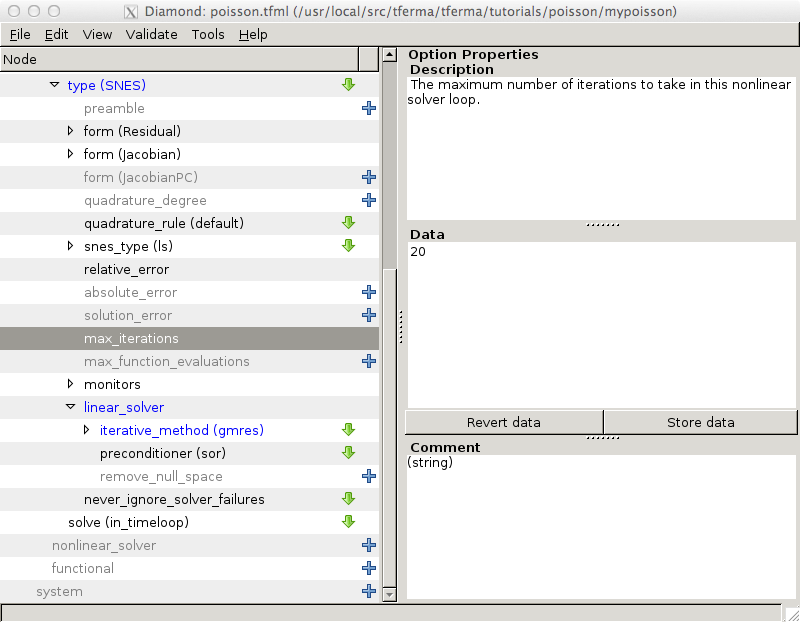
\includegraphics[width=\diamondwidth]{figures/screendumps/diamond_poisson_11e.png}
\end{center}
\item \textbf{Setting the Linear solver options:} Finally we need to
  set options for the inner linear solver.  For a small 2-D problem
  it's nearly impossible to beat sparse direct methods so we'll start
  with those.  Every linear solver has 2 components an
  \textbf{iterative\_method} (which is a PETSc KSP) and a
  \textbf{preconditioner} (a PETSc PC).  The appropriate (KSP,PC)
  pair for a direct solver is (preonly, lu), i.e a sparse-lu decomposition as
  a pre-conditioner (which is a direct solve) and no iterative
  method.  In \TF{} we use the green drop-down arrows to choose
  \textbf{linear\_solver} to be \texttt{preonly}, and
  \textbf{preconditioner} to be \texttt{lu}, which will default to the
  sparse direct solver \texttt{umfpack} (which is what is used in
  matlab).  Other direct solver packages such as mumps can also be chosen.
\begin{center}
    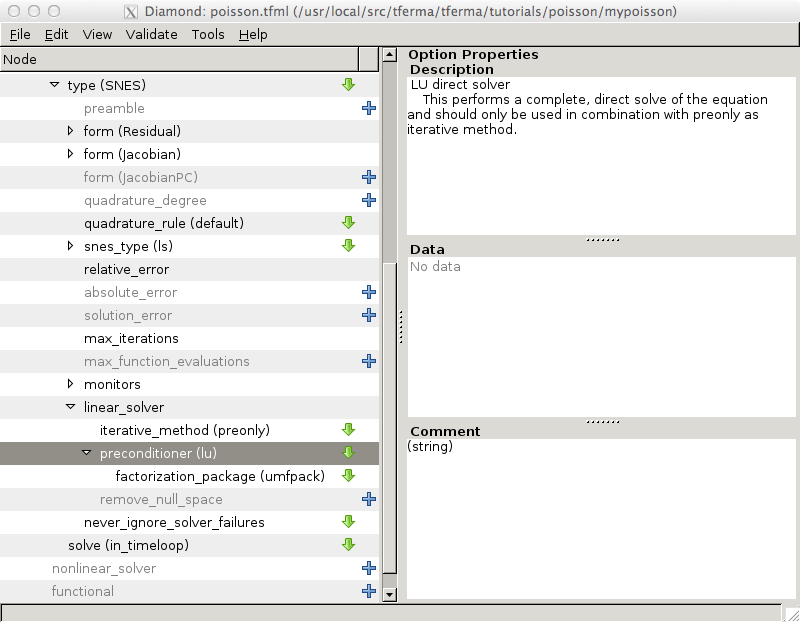
\includegraphics[width=\diamondwidth]{figures/screendumps/diamond_poisson_12a.png}
\end{center}
This completes all the choices required to build
\texttt{poisson.tfml}. \textbf{Save your file}, cross your fingers and see if
we can build this.
\item \textbf{Building and running your model:}  The instructions are
  given at the beginning of Section \ref{sec:ch2-solution-using-tf} but to
  repeat
\begin{lstlisting}[style=Bash]
$ tfbuild poisson.tfml
$ cd build
$ make run 
\end{lstlisting} %$
Compilation the first time requires automatic generation of C++ code from
the ufl forms (using FFC), then creating wrappers to link into the
base \TF{} libraries.  Once the code has been compiled however, changes
to run-time parameters will not force a recompile or relinking and
\lstinline[style=Bash]´$ make run´ %$
will be much quicker.  Any change to \texttt{ufl} or expressions that
require recompilation will force a rebuild automatically.
\item \textbf{Trouble shooting:} Murphy is the lord of modeling and
  anything that can go wrong will go wrong.  One of the nicer features
  of \TF{} is that it compartmentalizes many of the choices, which can
  help to more rapidly locate errors.  One of the poorer features of
  \TF{} is that the error messages are somewhat cryptic.

As a first cut,  use a good diff tool such as \texttt{meld} (Linux) or
\texttt{opendiff} (MacOSX) to compare your file \texttt{poisson.tfml} to
the working example in
\texttt{\$TF\_HOME/share/terraferma/tutorials/poisson/simple/poisson.tfml}.  You'll be
comparing raw \texttt{.tfml} (which is basically xml) but the diffs
should be small.  Simple things to watch out for are
\begin{itemize}
\item Make sure all the required fields are filled in (no blue fields)
\item Extra carriage returns in ufl symbols.
\item Syntax errors in ufl forms.  These errors will be generated
  during the code generation step by FFC.  Read the FFC output
  carefully to try and identify the problem.  The problem will most
  likely lie in the ufl for the weak forms of the residual (or Jacobian).
\item Syntax errors in python functions.  Some expressions can be
  written as small python functions.  If the python path is not set
  correctly or python errors are introduced, these will throw run-time errors.
\end{itemize}




 \end{steps}
  
%\lstinline[style=Bash]´$ tfbuild <filename>.tfml´.




\section{Themes and Variations}
\label{sec:themes-variations}

Given an initial working \texttt{tfml} file, one of the very nice
features of \TF{} is that it becomes usually quite straightforward to
rapidly change your choices to make new models or add new features.
\texttt{tfml} files are just ascii and can be copied to make new
files. In addition,  diamond allows entire options and option
sub-trees to be copied and pasted preserving (with some significant
care) work done in another model.  Here we will start by making some
small modifications to our basic working poisson model, then add some
advanced features such as including non-constant rhs's, boundary
conditions etc.

\subsection{Simple changes}
\label{sec:simple-changes}

Many changes simply change run-time options and have little to no
affect on other model options.  Some obvious ones include
\subsubsection{Changing Resolution}
\label{sec:changing-elements}

To increase the spatial resolution of the mesh, simply edit
\textbf{number\_cells} in the UnitSquare mesh and rerun.

\subsubsection{Changing the mesh}
\label{sec:changing-mesh}

Changing the mesh type itself may or may not be simple.  For example, changing to a rectangle
from a square only requires changing \textbf{source (UnitSquare)} to
\textbf{source (Rectangle)} and editing the appropriate
suboptions. Because the boundary IDs of a square and rectangle are
the same, however, this does not propagate to any other part of the
model. 
\begin{figure}[h!]
  \centering
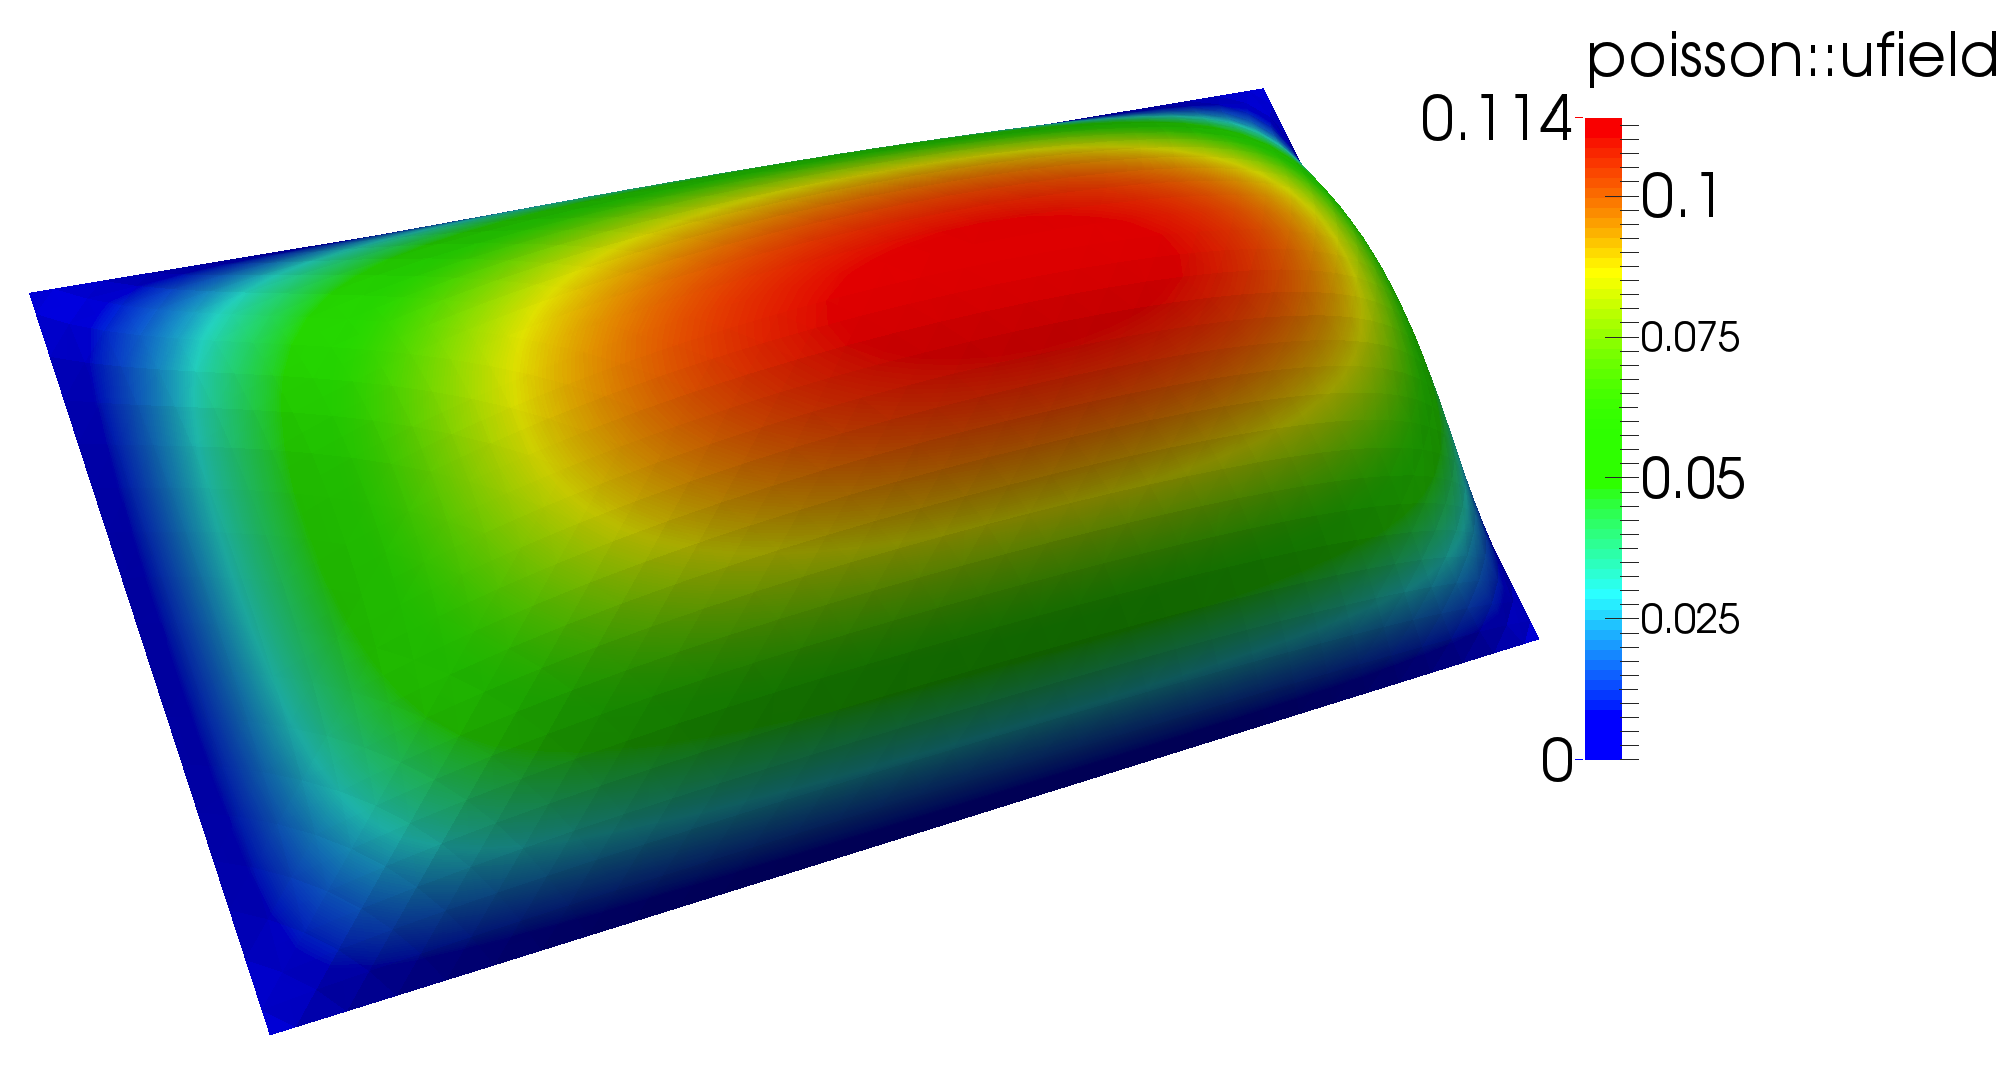
\includegraphics[width=.7\textwidth]{figures/poisson_simple_rectangle}
  \caption{\small Same problem but on a rectangular domain
    $\Omega=[0,2]\times[0,1]$ with $64\times32$ cells.}
\label{fig:poisson_rectangle}
\end{figure}

More generally, we would like to use externally generated meshes.  The
example \texttt{\$TF\_HOME/share/terraferma/tutorials/poisson/gmsh/poisson.tfml}
incorporates a mesh generated using \texttt{gmsh}.  The geometry file
for this mesh is in
\texttt{\$TF\_HOME/share/terraferma/tutorials/poisson/gmsh/mesh/widget.geo}. To convert
for use in TF (DOLFIN) use
\begin{lstlisting}[style=Bash]
$ cd $TF_HOME/share/terraferma/tutorials/poisson/gmsh/mesh
$ gmsh -2 -algo del2d widget.geo
$ dolfin-convert widget.msh widget.xml
\end{lstlisting}
the \texttt{gmsh} command generates a 2-D unstructured mesh in
\texttt{widget.msh} and  \texttt{dolfin-convert} generates a dolfin
meshfile in \texttt{.xml} format  that include the mesh geometry as
well as labels for boundary ids.  The actual boundary id's for the
exterior walls (1-6) and interior hole (7) can be found in the geometry file
\texttt{widget.geo}.

To incorporate this mesh into \texttt{poisson.tfml} we simply change
the mesh source to \texttt{Source (File)} and add the file name
relative to the \texttt{tfml} file (i.e. \texttt{../mesh/widget}
without the \texttt{.xml} extension). We also have to edit the
boundary id's in the boundary condition (and add one more boundary
condition for the hole).  A fully worked out example is included and
produces the result shown in Figure \ref{fig:poisson_gmsh}.
\begin{figure}[h!]
  \centering
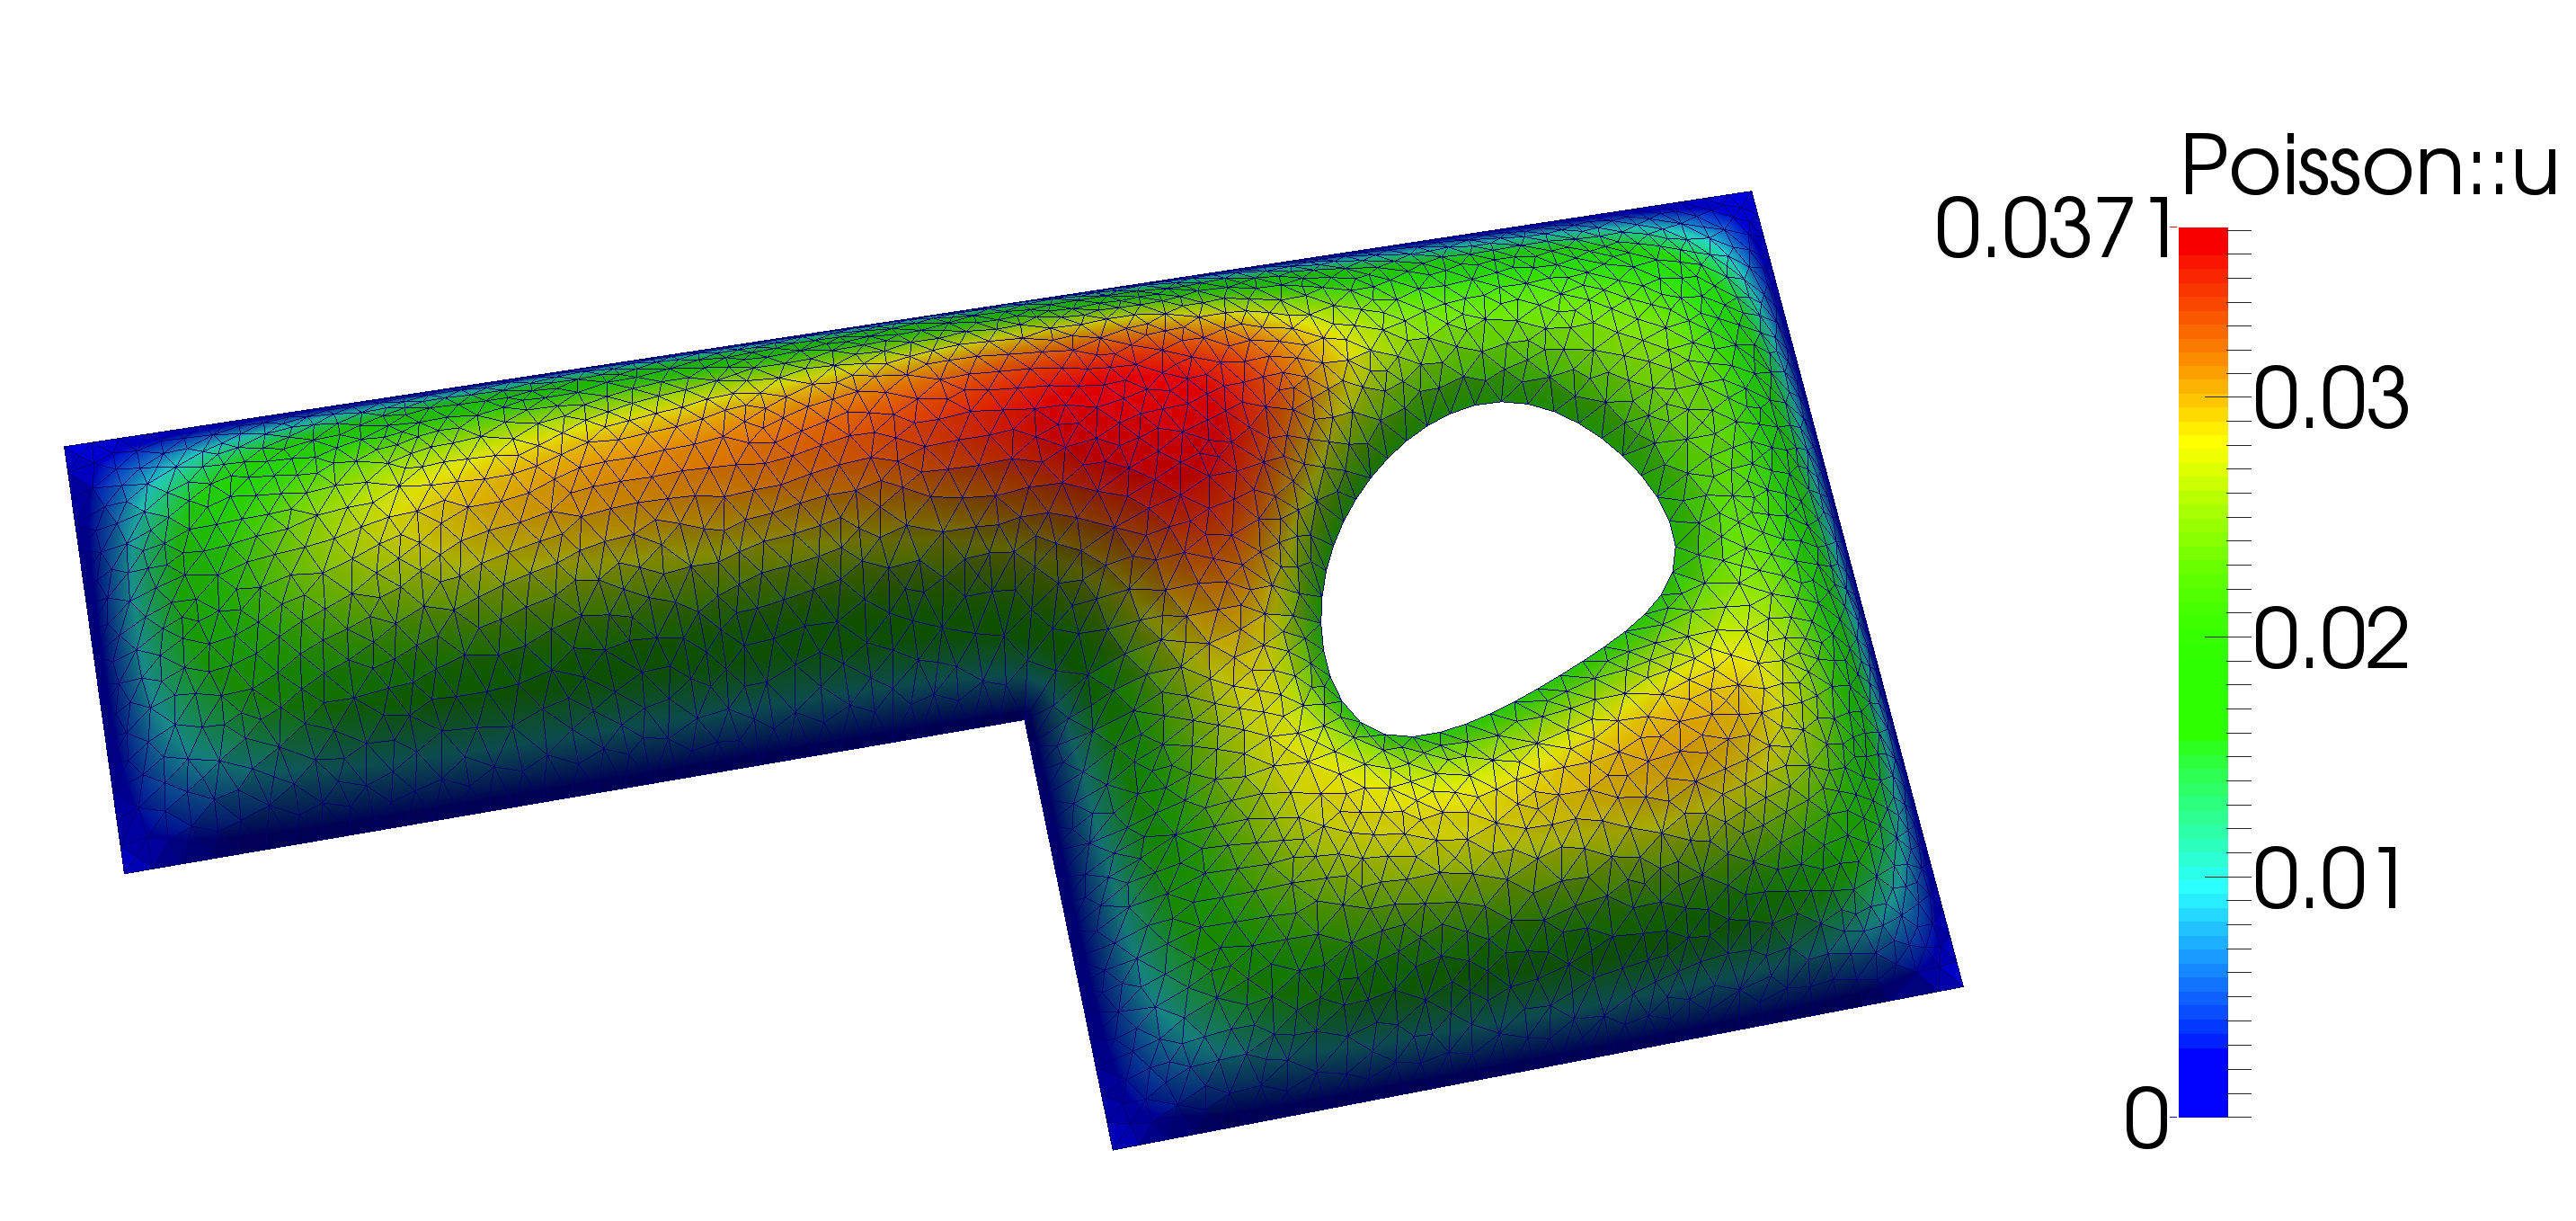
\includegraphics[width=.8\textwidth]{figures/poisson_simple_gmsh}
  \caption{\small Same problem but on an unstructured mesh generated using
    \texttt{gmsh}. Dirichlet boundary conditions for this problem are $u=0$ on
    the exterior faces and $u=0.02$ on the interior hole. }
\label{fig:poisson_gmsh}
\end{figure}

Alternatively, the mesh generation, model building and model execution
can be automated using the simulation testharness.  An example
testharness file, \texttt{poisson.shml} can be found in the gmsh
directory.  To run this file use
\begin{lstlisting}[style=Bash]
$ tfsimulationharness --test poisson.shml
\end{lstlisting}
%$
If all is successful,  the jobs will finish with
\begin{lstlisting}[style=Bash]
poisson.shml: Running tests:
poisson.shml: Running umax:
u_max = [0.037188591984999998]
poisson.shml: success.
poisson.shml: Running umin:
u_min = [0.0]
poisson.shml: success.
poisson.shml: PP
Passes:   2
Failures: 0
\end{lstlisting}


\subsubsection{Changing Elements}
\label{sec:changing-meshes}

Changing the order of an element is also trivial. For example
instead of P1 we could solve our initial problem using quadratic P2
elements by simply changing the \textbf{element} to (P2) under
\texttt{field} (i.e. Step 8).  To visualize these fields, however you
should also choose P2 as an element in
\textbf{io}$\rightarrow$\textbf{visualization}$\rightarrow$\textbf{element
(P2)}.  Changing the order of an element will force a recompile but
little else.
\begin{figure}[ht!]
  \centering
  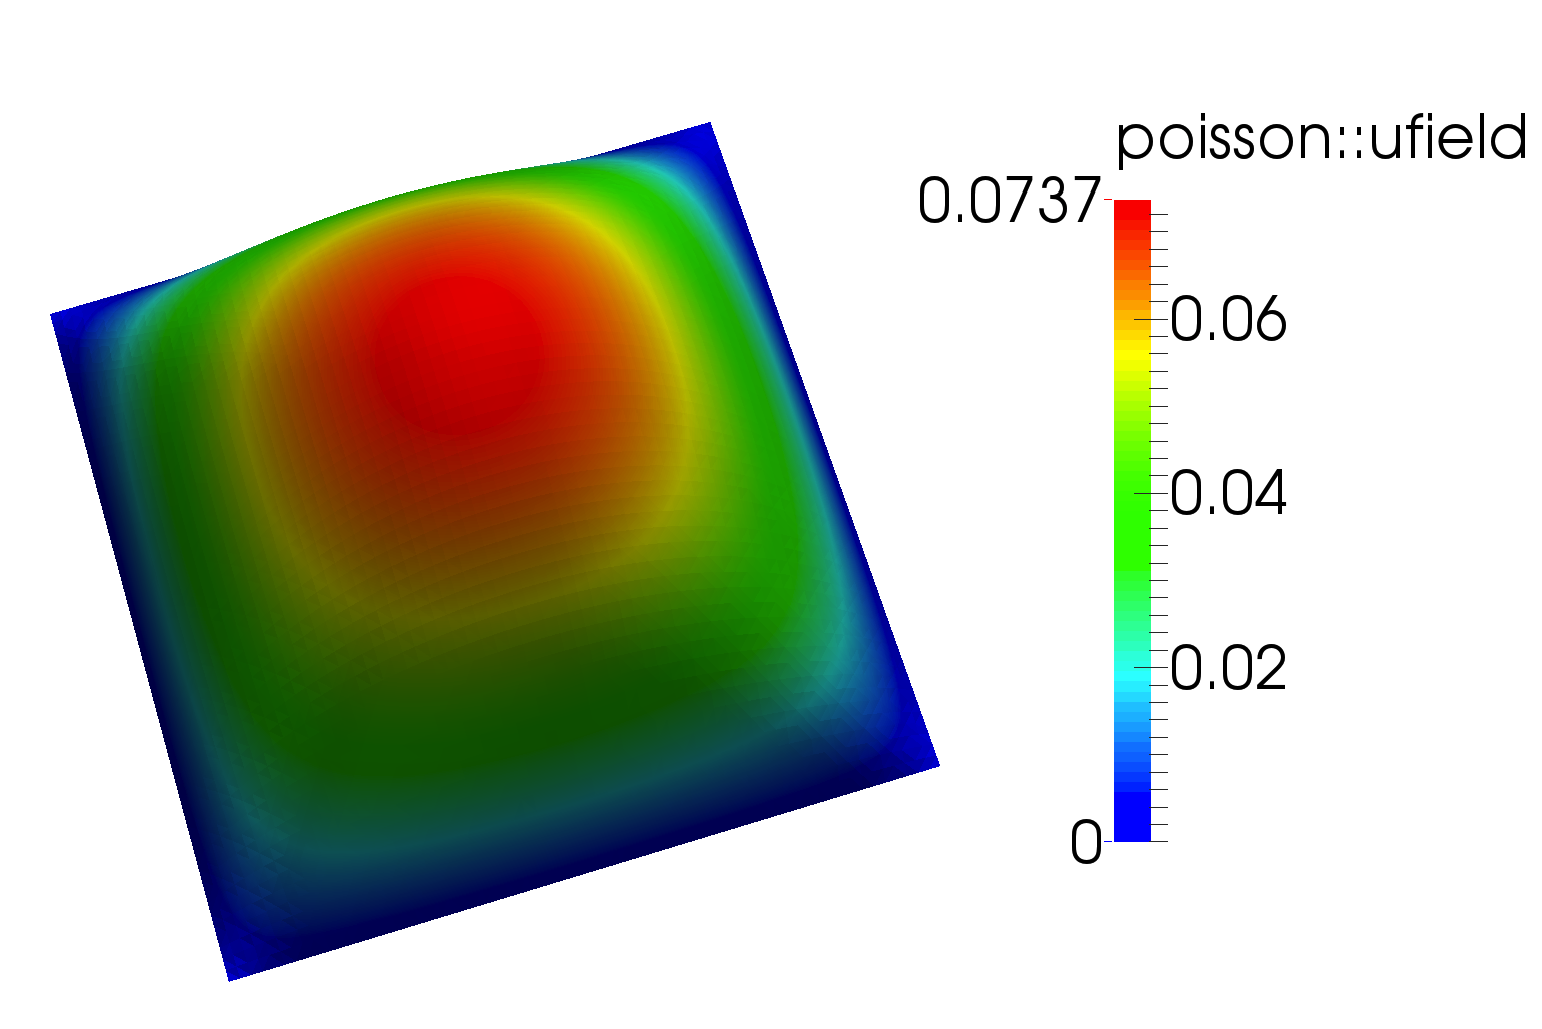
\includegraphics[width=.7\textwidth]{figures/poisson_simple_p2}
  \caption{Poisson problem with $32\times 32$ quadratic P2 elements and P2
    visualization. Compare to Figure \ref{fig:simple_poisson}}
  \label{fig:poisson-P2}
\end{figure}

To change elements entirely, for example to go with discontinuous
Galerkin (e.g. P2DG), is straightforward but forces changes to the
actual ufl for the weak form of the residual.

\subsubsection{Changing Solvers}
\label{sec:changing-solvers}

Changing solvers is straightforward as all PETSc solvers
allow choice of solvers and options at run-time.  For example, to
change from a direct solver (preonly,lu) to a algebraic-multi-grid
preconditioned conjugate gradient solver (cg,hypre) which is optimal
for poisson like problems, just edit the linear-solver to
\begin{lstlisting}[style=Bash]
iterative_method (cg)
   relative_error -> 1.e-7
   max_iterations -> 20
preconditioner (hypre)
\end{lstlisting}
If you want to exam the convergence behavior of the iterative linear
solve, simply turn on \textbf{monitors} and activate
\textbf{preconditioned\_residual}.  This will add convergence results
to the \texttt{terraferma.log-0} file which logs information about the run.
\begin{lstlisting}[style=Bash]
Solving for poisson::Solver using SNES
In FormFunction
In FormJacobian
    Residual norms for poisson_Solver_ solve.
    0 KSP Residual norm 1.249018252284e+00 
    1 KSP Residual norm 7.520968397518e-03 
    2 KSP Residual norm 1.054134570965e-04 
    3 KSP Residual norm 1.345208502264e-06 
    4 KSP Residual norm 2.609245158576e-08 
In FormFunction
Convergence for poisson::Solver
SNESConvergedReason 3
SNES n/o iterations 1
SNES n/o linear solver iterations 4
  KSPConvergedReason 2
  KSP n/o iterations 4
\end{lstlisting}
In addition, you can generate a \textbf{convergence\_file} that can be
interrogated using python scripts or provide quick visualization using
e.g.
\begin{lstlisting}[style=Bash]
$ tfplot poisson.conv
\end{lstlisting} %$
\begin{figure}[b!]
  \centering
  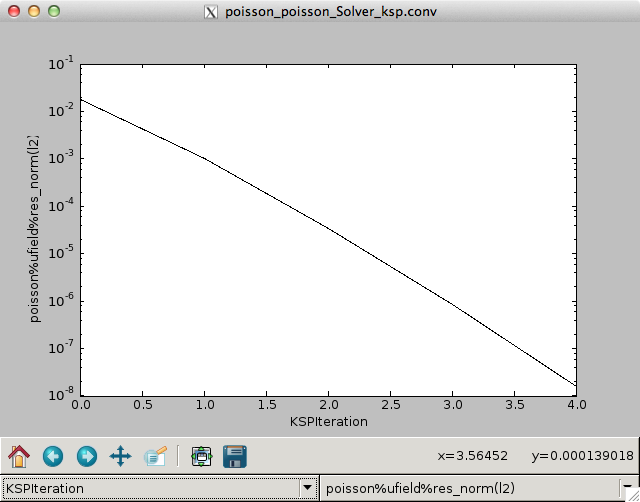
\includegraphics[width=.7\textwidth]{figures/screendumps/tfplot_cg-hypre-residuals.png}
  \caption{tfplot figure showing convergence rate of $||F||_2$ as a function of inner iteration for a (cg,hypre) iterative solver.}
  \label{fig:tfplot-convergence-poisson}
\end{figure}

{\samepage
The full \texttt{diamond} window for the linear solve should look like
\begin{center}
  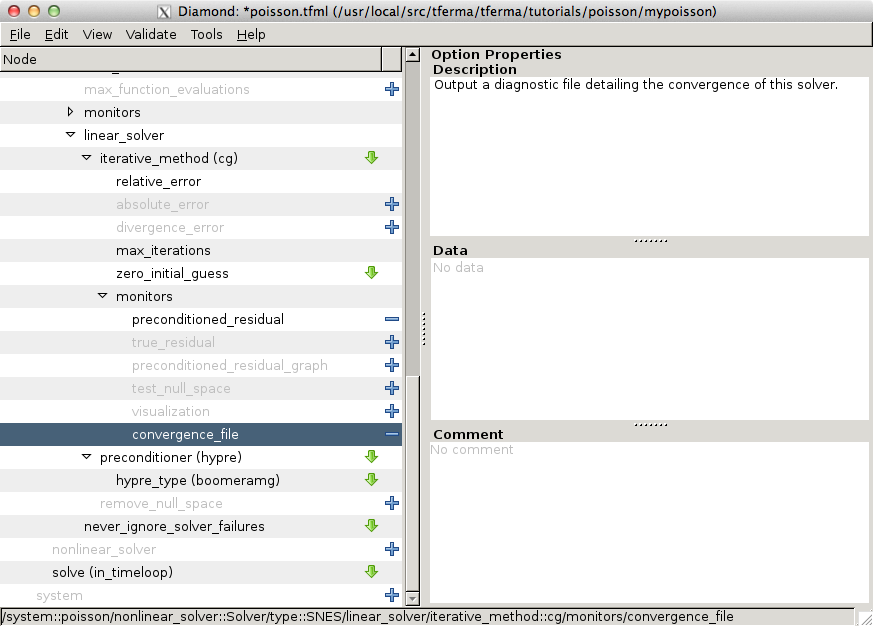
\includegraphics[width=\diamondwidth]{figures/screendumps/diamond_poisson_cg-hypre.png}
\end{center}
}

\subsubsection{Changing Dimensions}
\label{sec:changing-dimensions}

Changing dimensions is slightly more difficult, but only due to a
design issue with \texttt{diamond} which only lets you set the
dimension of the problem once.  For a basic poisson problem, it is not
difficult to simply start from scratch (or with some caution, try
editing the \texttt{.tfml} file directly). The only changes being to
\texttt{dimension} (Step 3) , \texttt{source (UnitCube)} (and
suboptions) (Step 4)  and
add additional \textbf{boundary\_ids} (Step 10).  You should also
probably change the solver to an iterative solver (e.g. (cg,hypre) or (cg,ml)) as
sparse direct solvers become significantly more expensive in memory
and time in 3-D.  A fully worked example \texttt{tfml} file can be
found in \texttt{tutorials/poisson/simple\_3d}.
Convergence behavior of the SNES and KSP is
\begin{lstlisting}[style=Bash]
Solving for Poisson::SNES using SNES
In FormFunction
  0 SNES Function norm 5.267355201652e-03 
In FormJacobian
    Residual norms for Poisson_SNES_ solve.
    0 KSP Residual norm 4.316879223510e+00 
    1 KSP Residual norm 2.742504639453e-02 
    2 KSP Residual norm 3.692535718352e-04 
    3 KSP Residual norm 4.750897104741e-06 
    4 KSP Residual norm 7.029490501627e-08 
    5 KSP Residual norm 1.289791412984e-09 
    6 KSP Residual norm 1.877399607342e-11 
In FormFunction
  1 SNES Function norm 4.727883538082e-13 
Convergence for Poisson::SNES
SNESConvergedReason 3
SNES n/o iterations 1
SNES n/o linear solver iterations 6
  KSPConvergedReason 2
  KSP n/o iterations 6
\end{lstlisting}
\begin{figure}[ht!]
  \centering
  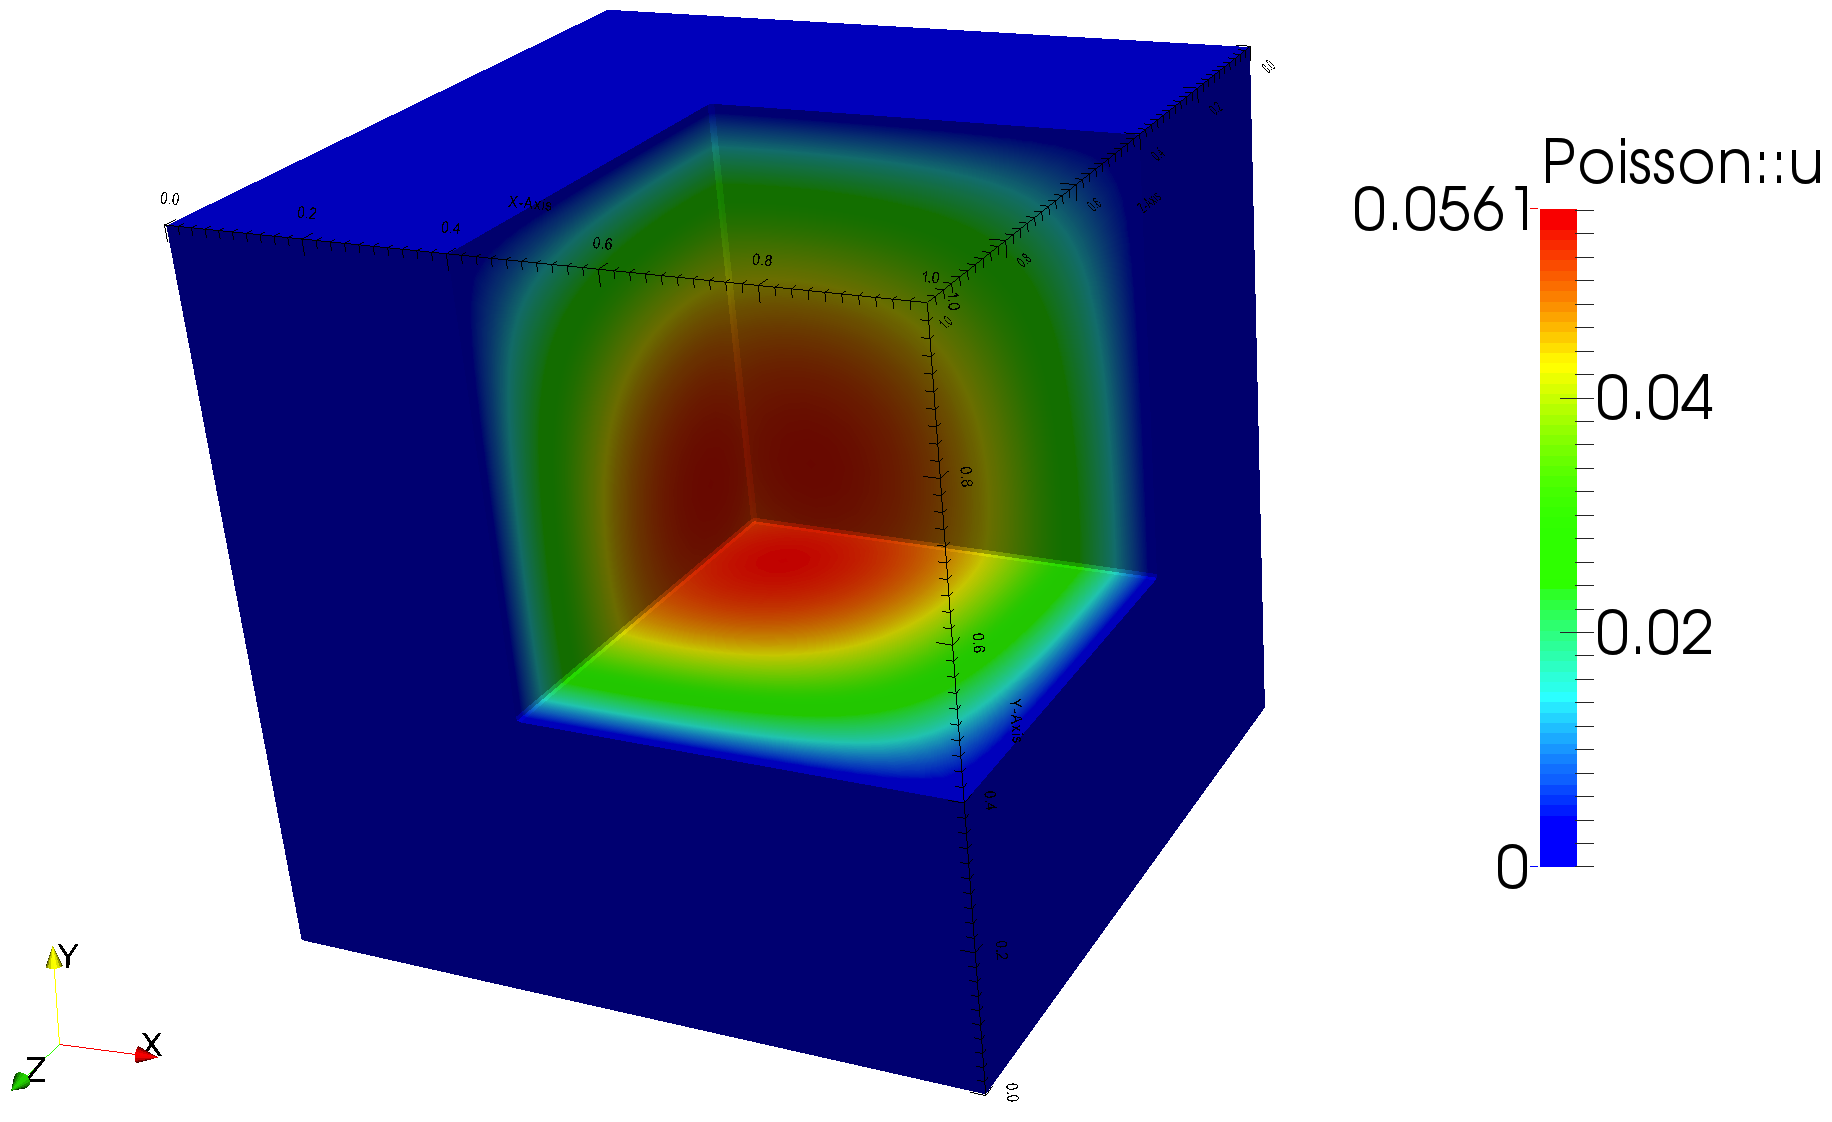
\includegraphics[width=.7\textwidth]{figures/poisson_simple_3d}
  \caption{3D poisson problem on a unit cube with unit forcing and homogeneous $u=0$ BC's}
  \label{fig:poisson-3D}
\end{figure}

\pagebreak
\subsection{Adding variable coefficients: Manufactured Solutions}
\label{sec:manuf-solut}

The basic Poisson problem with unit forcing is a useful first example,
and in fact has a (very slowly converging) spectral solution with
which we could test the accuracy of our Finite Element Model.
However, a more useful approach for testing numerical solutions is the
\emph{method of manufactured solutions}, where we simply choose a
solution $u$ and determine a forcing term $f$ and boundary conditions
that are consistent with that solution.  One particular manufactured
solution for Poisson is given in Leveque's excellent book on finite
difference methods \cite{leveque_finite_2007} which is simple (if
visually uninspiring)
\begin{equation}
  \label{eq:13}
  u_{mms}(x,y) = \exp(x + y/2)
\end{equation}
with
\begin{equation}
  \label{eq:14}
  -\nabla^{2} u_{mms} = -\frac{5}{4}\exp(x+y/2)
\end{equation}
and
\begin{equation}
  \label{eq:15}
  \grad u_{mms} = \exp(x+y/2)
  \left[
    \begin{array}{c}
 1 \\
1/2\\
\end{array}
  \right]
\end{equation}

Given the solution we can recast the problem (and now include  Neumann boundary conditions) as,
\begin{align}
  \label{eq:16}
-\nabla^2u &= f \quad\text{in } \Omega=[0,1]\times[0,1] \nonumber\\
\grad u\cdot\vec{n} & = g \quad\text{on } \partial\Omega_{N}=(x=1)\\
 u &= h \quad\text{on } \partial\Omega_{D}\nonumber
\end{align}
with  prescribed functions
\begin{align}
  \label{eq:17}
  f &= -\frac{5}{4}\exp(x+y/2)\nonumber\\
  g & = \exp(x+y/2)\\
  h &=  \exp(x+y/2)\nonumber
\end{align}
where $\partial\Omega_{N}$ are Neumann boundaries (here the right side
of the box at $x=1$) and $\partial\Omega_{D}$ are the remaining Dirichlet boundaries (top, bottom,and left).

The weak form of the residual after integration by parts (and
including the surface terms) now looks like
\begin{equation}
  \label{eq:4}
  F(u_{i};u_{t}) = \int_{\Omega}
  \left(
    \grad u_{t}\cdot\grad u_{i} - u_{t}f
  \right)dx - \int_{\partial\Omega_{N}} u_{t}g ds
\end{equation}
or in ufl
\begin{lstlisting}[style=ufl]
F = (inner(grad(u_t),grad(u_i)) - u_t*f)*dx - u_t*g*ds(2)
\end{lstlisting}
where \texttt{ds(2)} implies a surface integral along boundary id 2
(right hand side for our unit square). Implementing this problem now
requires us to input variable forcing and boundary coefficients
$(f,g)$ in the form as well as impose variable Dirichlet conditions on
the other walls.

Adding variable Coefficients as FEniCS \emph{expressions} is
relatively straightforward in \TF{}. They can be included as small
python functions (which can be slow in large calculations) or as C++
expressions.  Here we will just demonstrate the python interface.  A
fully worked out example is in \texttt{tutorials/poisson/mms/poisson.tfml}.

To add these new features (and visualize the error from the analytic solution), do the following.
\begin{steps}{Step}
\item  Start with the simple poisson.tfml
  \begin{lstlisting}[style=Bash]
$ mkdir mymms
$ cd mymms
$ cp $TF_HOME/share/terraferma/tutorials/poisson/simple/poisson.tfml .    
  \end{lstlisting}
\item Change the coefficient \texttt{f} in \textbf{system (Poisson)} to a python Expression. Unfold the \textbf{coefficient (f)} tab until you see the Expression value as \textbf{constant}. 
\begin{center}
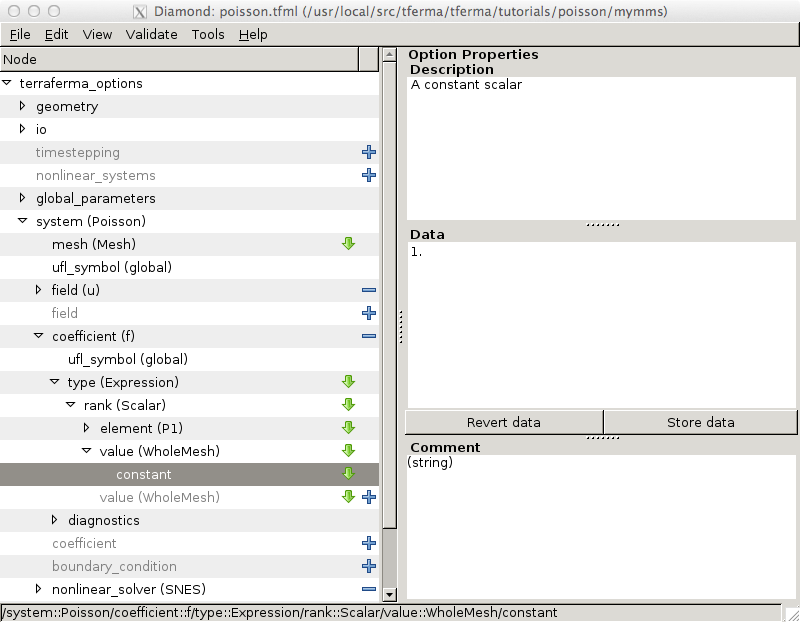
\includegraphics[width=\diamondwidth]{figures/screendumps/diamond_poisson_f_value.png}
  \end{center}
\item using the drop down menu, change the value from \textbf{constant} to \textbf{python} and in the data window, replace \texttt{(string)} with the following small python function
  \begin{lstlisting}[style=python]
from math import exp
def val(x):
  global exp
  return -5./4.*exp(x[0] + x[1]/2.)   
  \end{lstlisting}
(and be careful about the indentation). \texttt{f} is now a variable coefficient which will return $f(\vec{x}) = -5/4(\exp(x + y/2)$ at any point $\vec{x}$. Your diamond window should now look like
\begin{center}
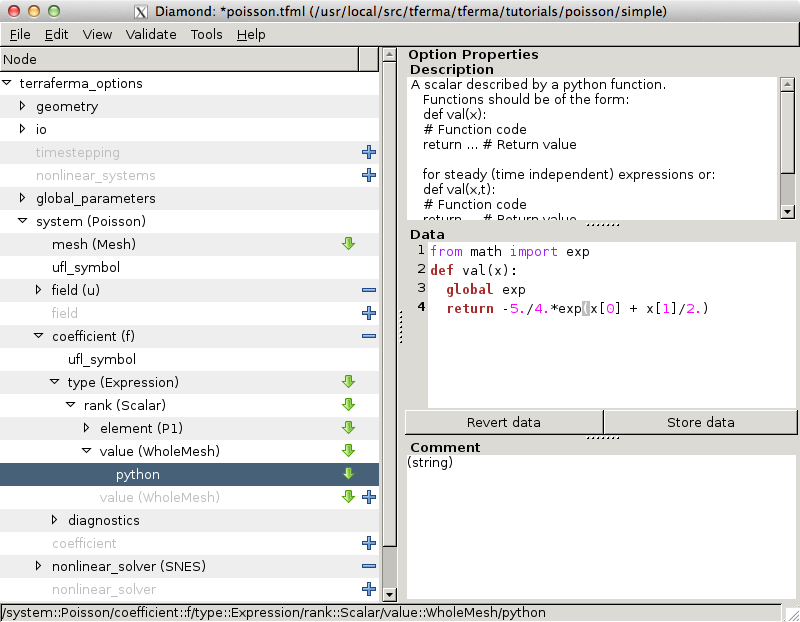
\includegraphics[width=\diamondwidth]{figures/screendumps/diamond_poisson_mms_f_value.png}
  \end{center}
\item \textbf{Change the Dirichlet Boundary conditions}.  Under \textbf{field (u)}$\rightarrow$\textbf{type (Function)}, find and unfold the \textbf{boundary\_condition (homogeneous)} tab.  Select \textbf{boundary\_ids} and remove \texttt{2} (right boundary) from the list to leave \texttt{1 3 4}.  Then unfold \textbf{sub\_components (All)}$\rightarrow$\textbf{type (Dirichlet)} and change the value from \textbf{constant} to \textbf{python} and add the python function
\begin{lstlisting}[style=python]
from math import exp
def val(x):
  global exp
  return exp(x[0] + x[1]/2.)    
\end{lstlisting}
\begin{center}
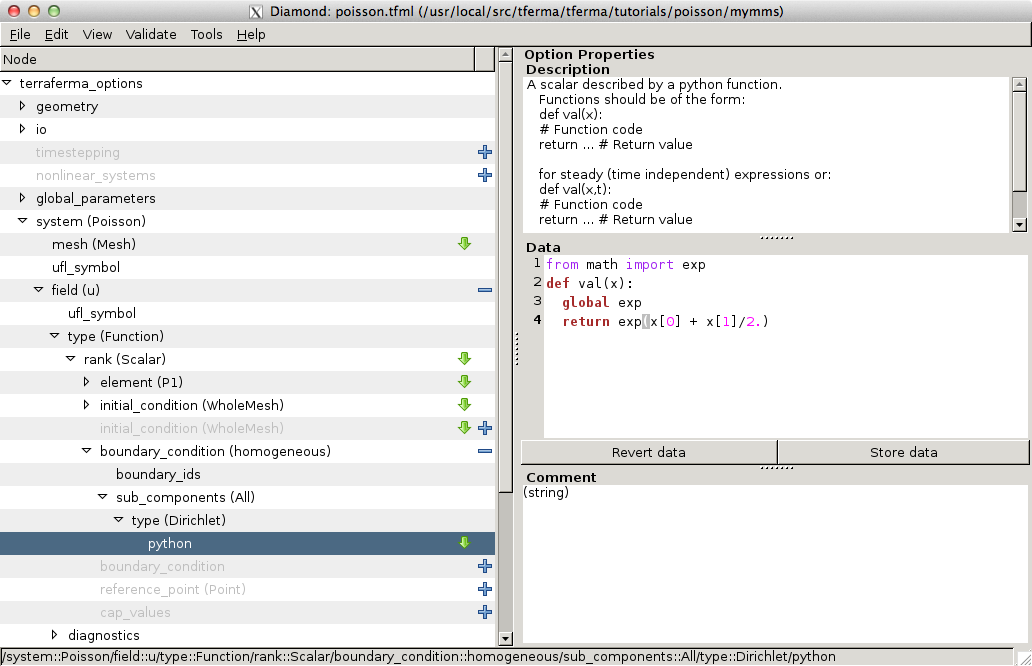
\includegraphics[width=\diamondwidth]{figures/screendumps/diamond_poisson_mms_bcs.png}
  \end{center}
\item \textbf{Add a new coefficient (g)} for the Neumann boundary conditions.  The cleanest way to do this is to activate a new coefficient tab and set the \texttt{name} and \textbf{ufl\_symbol} to \texttt{g},  the \textbf{element} to \texttt{P1} and the \textbf{value (WholeMesh)} to \textbf{python} and add the python function
\begin{lstlisting}[style=python]
from math import exp
def val(x):
  global exp
  return exp(x[0] + x[1]/2.)    
\end{lstlisting}

The slightly dangerous, but quicker way is to use the copy and paste
features of \texttt{diamond} where you can copy and paste entire
sub-trees of options, i.e. select the top tab \texttt{coefficient
  (f)}, and using the edit menu select \texttt{Copy}, then activate a
new coefficient tab and select \texttt{Paste}.  This should give you a
copy of the entire options tree of the \textbf{coefficient (f)}.  You
now just have to edit the coefficient \texttt{name} and
\textbf{ufl\_symbol (global)} to \texttt{g}, and edit the \textbf{python} function to the listing above. 
 \begin{center}
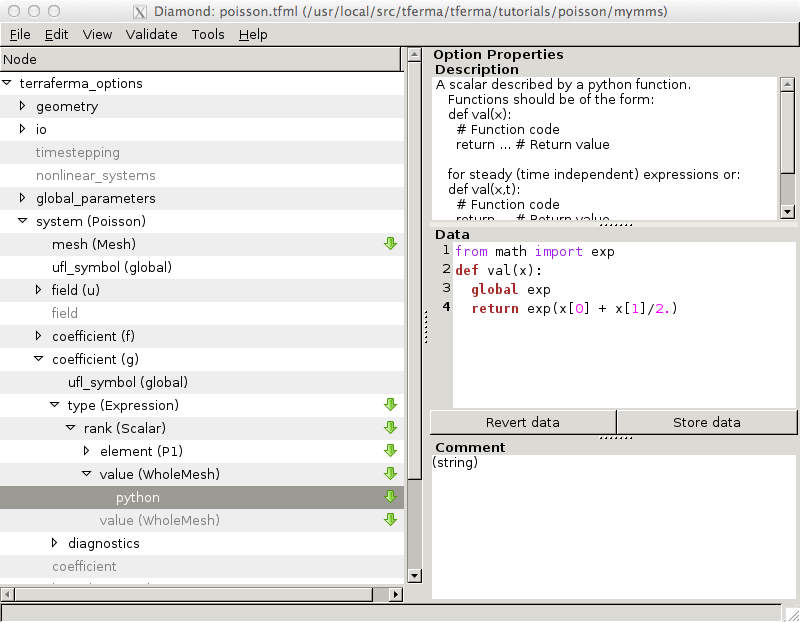
\includegraphics[width=\diamondwidth]{figures/screendumps/diamond_poisson_mms_g_value.png}
  \end{center} 
\item \textbf{Edit the UFL for the residual}. We now have to add the boundary terms for \texttt{g} into the residual equations.  Unfold \textbf{nonlinear\_solver (SNES)}$\rightarrow$\textbf{type (SNES)} and choose \textbf{form (Residual)}, and change
  \begin{lstlisting}[style=UFL]
    F = (inner(grad(u_t),grad(u_i)) - u_t*f)*dx
  \end{lstlisting}
to
  \begin{lstlisting}[style=UFL]
    F = (inner(grad(u_t),grad(u_i)) - u_t*f)*dx - u_t*g*ds(2)
  \end{lstlisting}
\begin{center}
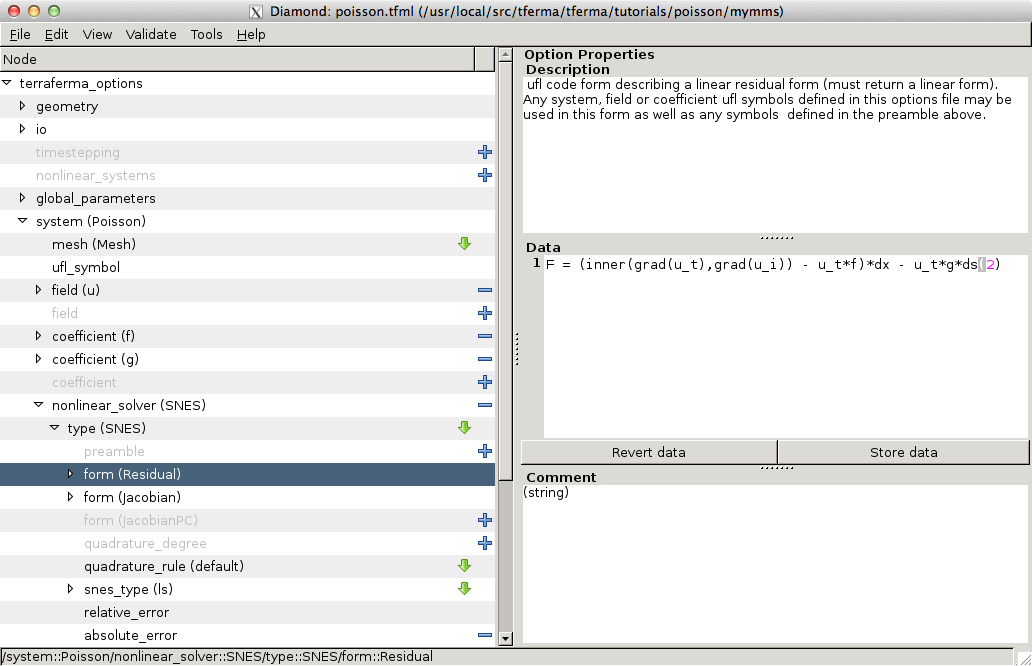
\includegraphics[width=\diamondwidth]{figures/screendumps/diamond_poisson_mms_residual.png}
  \end{center}
\item At this point you should be able to build and run the new model
  \begin{lstlisting}[style=Bash]
$ tfbuild poisson.tfml
$ cd build
$ make run
   \end{lstlisting} %$
and it should look something like
\begin{figure}[h]
  \centering
  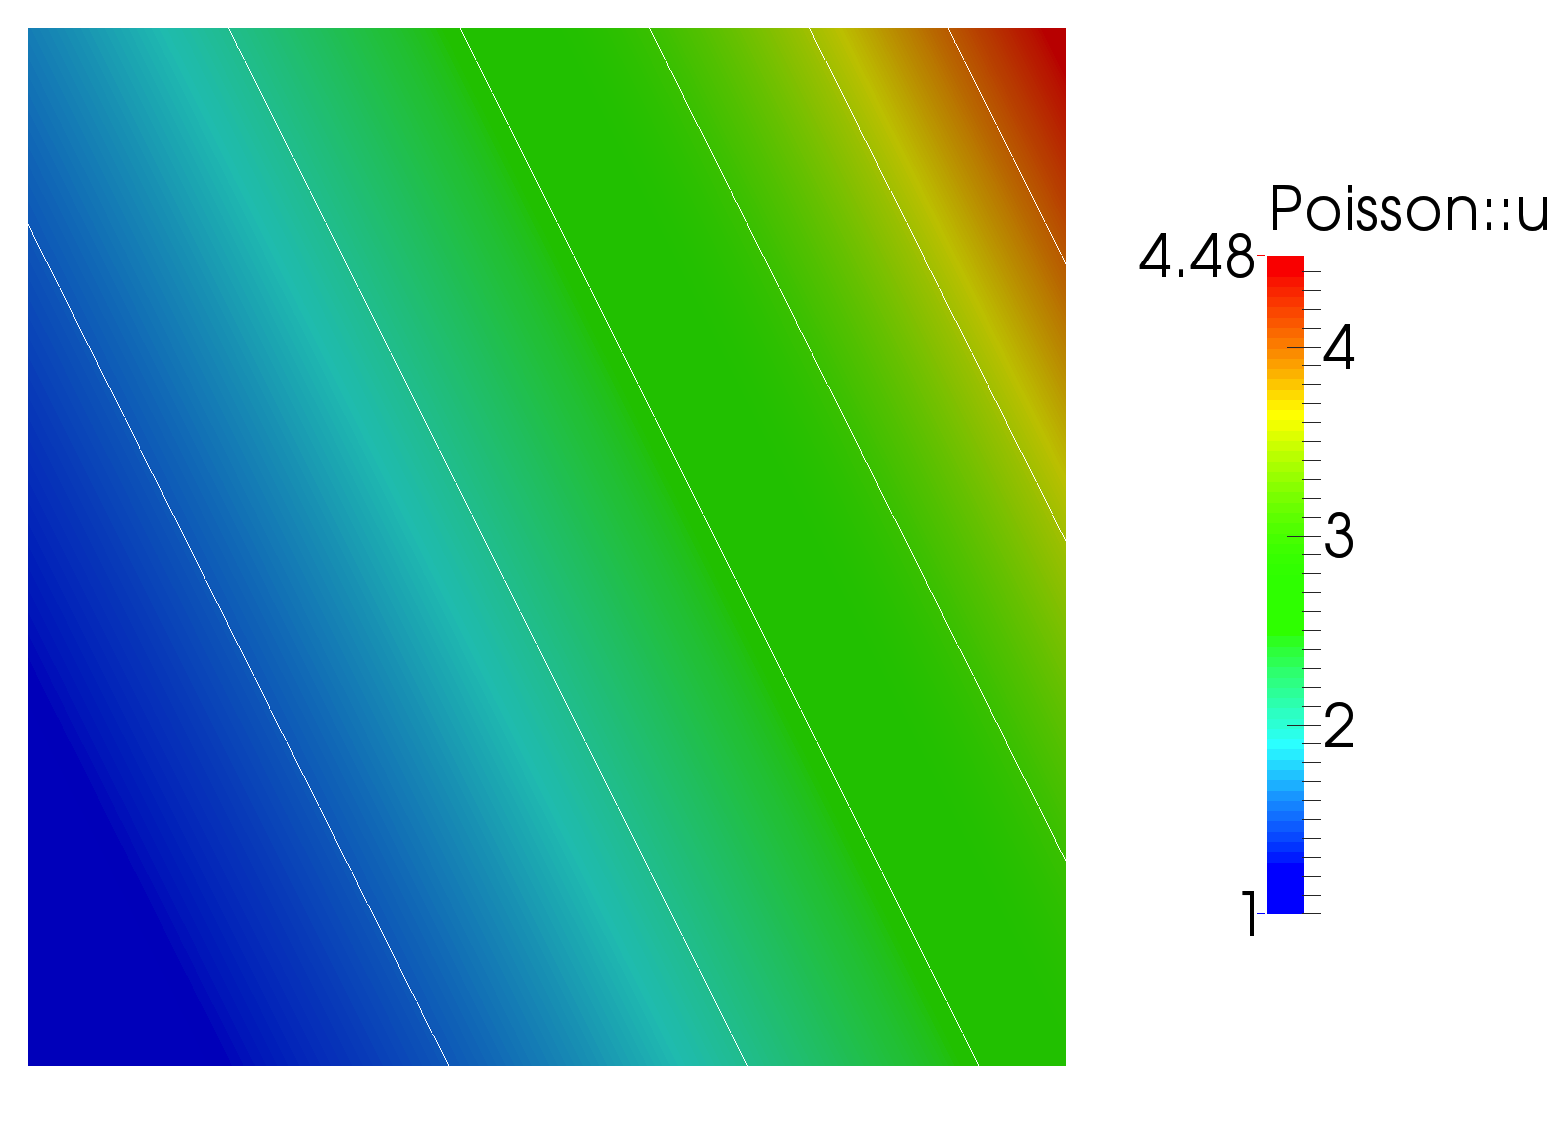
\includegraphics[width=.7\textwidth]{figures/poisson_mms.png}
  \caption{solution for the Poisson mms example (not terribly exciting looking)}
  \label{fig:poisson_mms}
\end{figure}

\end{steps}

\paragraph{Adding Error monitoring}
\label{sec:adding-error-monit}

Pretty pictures are nice,  but the whole point of MMS is that we can
calculate the exact error to test our solutions as well as
convergence.  The example program
\texttt{\$TF\_HOME/share/terraferma/tutorials/poisson/mms/poisson.tfml} has two
mechanisms for calculating and monitoring the absolute error of this
solution.  One simple approach is just to  visualize errors by
creating a new system that calculates the projection of $e = u -
u_{exact}$ onto the Function Space P1 and outputting this solution for
visualization.  The example \texttt{poisson.tfml} includes this
additional system.

An alternate approach, however is to calculate a functional
\begin{equation}
  \label{eq:18}
  e^{2} = \int_{\Omega} (u-u_{exact})^{2} dx
\end{equation}
which is the square of the L2 norm of the absolute error and output it
to statistics for later processing.  To implement this
\begin{steps}{Step}
\item First create another coefficient by copying \textbf{coefficient (g)} then changing the name to \texttt{AnalyticSolution} and \textbf{ufl\_symbol} to \texttt{ue}.  The python to evaluate \texttt{g} and the analytic solution are the same (coincidentally).
\item \textbf{Add a functional to the system} Next we have to attach a
  functional to the system  and output to statistics.  Do the following
  \begin{steps}{step}
  \item activate the greyed out tab \textbf{functional} and give it a \textbf{name} (L2NormErrorSquared) and a piece of ufl to evaluate the functional in Eq.\ (\ref{eq:18})
    \begin{lstlisting}[style=UFL]
e2 = ( u - ue )**2 *dx
    \end{lstlisting}
  \item set the  \textbf{ufl\_symbol} for the functional to \texttt{e2}
  \end{steps}
\end{steps}
\begin{center}
    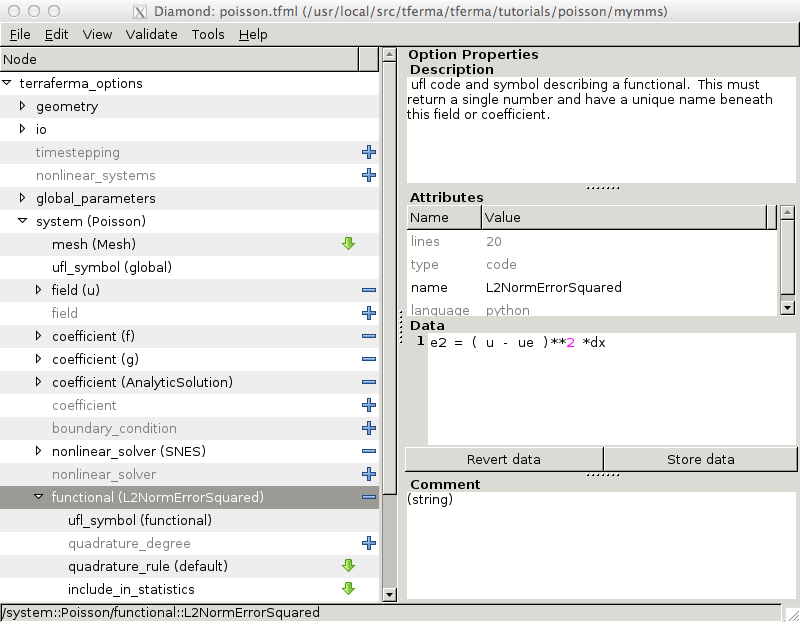
\includegraphics[width=\diamondwidth]{figures/screendumps/diamond_poisson_mms_functional.png}
\end{center}
The value of the functional will now be written to the statistics file
\texttt{poisson.stat} as part of a python dictionary that can be
either viewed with \texttt{tfplot} or interrogated using additional
python modules furnished with \TF{}.

\paragraph{Running parameter sweeps using the simulation test-harness}
\label{sec:runn-param-sweeps}

To calculate convergence for this mms problem requires running our
basic \texttt{.tfml} file for a range of mesh sizes, accumulating the
errors for each mesh file and producing output (e.g. a convergence
plot such as Figure \ref{fig:poisson_convergence} ).  To aid in
running multiple simulations or parameter sweeps as well as providing
a uniform testing environment for regression testing of \TF,  we have
also developed the \emph{TerraFERMA simulation test-harness}. 

While an individual \texttt{.tfml} file records all the options
required for a single instance of a model, a test harness options file
(with extension
\texttt{.shml}  for simulation harness markup language), controls the
work flow for building, running and testing multiple models as well as
handling dependencies such as mesh generation.   We have included an example in
\texttt{\$TF\_HOME/share/terraferma/tutorials/poisson/mms/poisson.shml},
that takes as input  the tfml file \texttt{poisson.tfml}  and runs a
parameter sweep over the mesh parameter \texttt{ncells}, but using the
python bindings to the spud library (libspud) to generate a directory
structure and a set of individual \texttt{tfml} files for each model.
In addition,  the test harness will build a single copy of the binary,
run multiple versions of the model,  collect error information for
each grid spacing and plot the convergence behavior.  It will also
provide a test to make sure that the  MMS problem show the expected
quadratic convergence.

To view the testharness file use
\begin{lstlisting}[style=Bash]
 $ diamond poisson.shml
\end{lstlisting} %$
To run it, we use the utility function
\texttt{tfsimulationharness}.  Options for tfsimulationharness are
provided using 
\begin{lstlisting}[style=Bash]
$ tfsimulationharness -h
\end{lstlisting} %$
% usage: tfsimulationharness [-h] [-n NTHREADS] [-r [depth]] [-l length [length ...]] [-p parallelism] [-o ownerid [ownerid ...]] [-t tag [tag ...]] [-e tag [tag ...]] [--generate] [--configure] [--build] [--run] [--test]
%                            [--just-test] [--just-list] [--list-input] [--clean] [-f]
%                            filename [filename ...]
%
% Run simulations and manipulate the output data.
%
% positional arguments:
%   filename              specify filename(s)
%
% optional arguments:
%   -h, --help            show this help message and exit
%   -n NTHREADS, --nthreads NTHREADS
%                         number of threads
%   -r [depth], --recursive [depth]
%                         recursively search the directory tree for files (if no depth is specified full recursion will be used)
%   -l length [length ...], --length length [length ...]
%                         length(s) of problem (if unspecified will run all lengths)
%   -p parallelism, --parallelism parallelism
%                         parallelism of problem: options are serial, parallel or any (default=any)
%   -o ownerid [ownerid ...], --owner ownerid [ownerid ...]
%                         run only tests that have specific owner ids (if unspecified will include all owners)
%   -t tag [tag ...], --tags tag [tag ...]
%                         run only tests that have specific tags (if unspecified will run all tags)
%   -e tag [tag ...], --exclude tag [tag ...]
%                         run only tests that do not have specific tags (takes precedence over -t, if unspecified will not exclude any tags)
%   --generate            generate the simulation directories and input
%   --configure           configure the simulations
%   --build               build the simulations
%   --run                 run the simulations
%   --test                test the simulations
%   --just-test           only test the current output of the simulations (do not rerun)
%   --just-list           only list the simulations
%   --list-input          list the input to the simulations
%   --clean               removes the run (and build) directories from previous simulation runs
%   -f, --force           force rebuild(s)
% \end{lstlisting} %$
which provides considerable flexibility in building, running and
testing specific applications. More details on the testharness and
other \TF{} utilities can be found on the \TF{}
\href{https://terraferma.github.io}{Wiki} under additional tools.

To build, run and test the example mms problem just
\begin{lstlisting}[style=Bash]
$ cd mms
$ tfsimulationharness --test poisson.shml
\end{lstlisting} %$
which will generate two directory structures:
\texttt{poisson.tfml.build} contains the binary file and
\texttt{poisson.tfml.run} contains a set of sub-directories for each
individual run labeled by the parameter (in this case
\texttt{ncells\_8}, \texttt{ncells\_16}, etc.).   Using the
\texttt{--test} option, it will also calculate the best-fit degree of
accuracy (which should be $p=2$ for a second order accurate problem in
$P_1$) and check that it is greater than 1.9.  It will also use
matplotlib to produce the pdf file shown in  Figure
\ref{fig:poisson_convergence}.

Output of a successful run should look like
\begin{lstlisting}[style=Bash]
poisson.shml: Running tests:
poisson.shml: Running error_l2_p1:
OrderedDict([('ncells', ['8', '16', '32', '64', '128'])])
***********  order of accuracy p= 1.98737547825
***********  convergence figure in poisson_convergence.pdf
poisson.shml: success.
poisson.shml: P
Passes:   1
Failures: 0
\end{lstlisting}

\begin{figure}[ht!]
  \centering
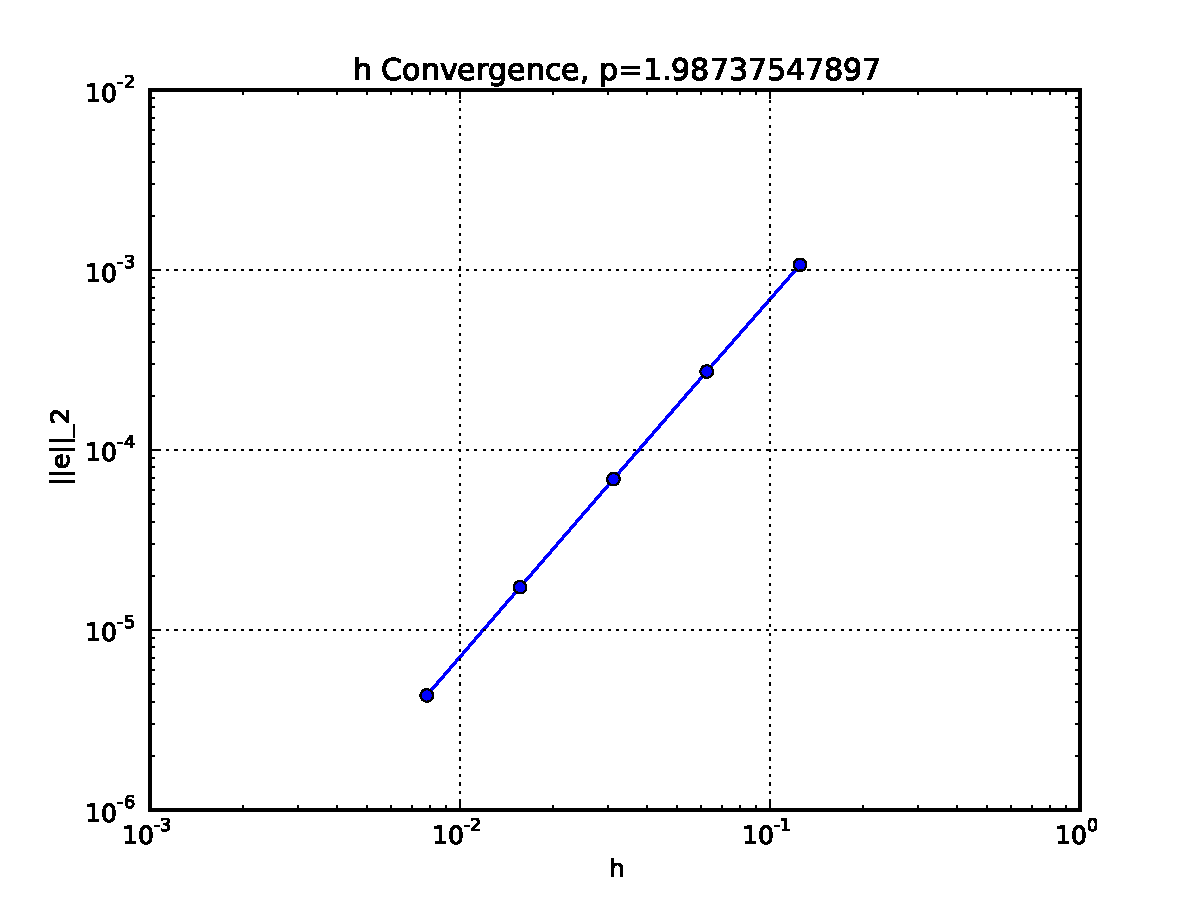
\includegraphics[width=.6\textwidth]{figures/poisson_convergence.pdf}
  \caption{Convergence plot for poisson mms problem. $h=1/N$ is the nominal grid spacing}
  \label{fig:poisson_convergence}
\end{figure}






%%% Local Variables: 
%%% mode: latex
%%% TeX-master: "tftutorials"
%%% End: 
